% \listfiles
\documentclass[a4paper]{article}
\usepackage[T2A]{fontenc}
\usepackage[english,russian]{babel}
\usepackage{sectsty}
\sectionfont{\centering\normalfont}
\subsectionfont{\centering\normalfont}
\subsubsectionfont{\normalfont}
\usepackage{changepage}
\usepackage{filecontents}
% \usepackage{mathptmx}
\usepackage{float} 
\usepackage{subcaption}
\usepackage[utf8]{inputenc}
\usepackage[14pt]{extsizes}
\usepackage{physics} 
\usepackage{graphicx}
\usepackage{enumerate}
\graphicspath{{../misc/}}
\usepackage{setspace,amsmath}
% \usepackage[left=30mm, right=15mm, top=20mm, bottom=20mm]{geometry} 
\usepackage[nottoc]{tocbibind}
\usepackage[style=gost-numeric,sorting=none,backend=biber,defernumbers=false]{biblatex}
\DeclareBibliographyAlias{misc}{article}
\addbibresource{lit.bib} 
%%%%%%%%%%%%%%%%%%%%%%%%%%%%%%%%%%%%%
% \everymath{\displaystyle}
\DeclareMathSizes{12}{20}{14}{10}

\makeatletter
\def\@makefnmark{\hbox{\@textsuperscript{\normalfont(\@thefnmark)}}}
\makeatother
 
\captionsetup[figure]{labelsep=period}
\captionsetup[table]{labelsep=period}

\usepackage{titling,lipsum}

\usepackage{amsmath}
\usepackage{bm}

\usepackage{hyperref}
\hypersetup{
    colorlinks,
    citecolor=black,
    filecolor=black,
    linkcolor=black,
    urlcolor=blue
}

\begin{document}

\thispagestyle{empty}

\begin{center}
    \large\textbf{Training competition connections between local receptive fields in spiking neural networks}\\
    \hfill\break
    
    Daniil Gafni, Dmitry Nekhaev, Vyacheslav Demin
\end{center}


% \tableofcontents


% \pagebreak

\addcontentsline{toc}{section}{Abstract}
\section*{Abstract}
Standard learning methods (based on the error backpropagation) used in formal artificial neural networks (ANNs) are difficult to apply to spiking neural networks (SNNs) due to discrete and time-distributed nature of the events they generate --- impulses, or spikes. Although such projects exist, local learning algorithms, which are more biologically correct, capable of performing unsupervised learning (without a teacher) and more energy efficient (if implemented on specialized hardware), are of greater interest.

One of the main disadvantages of the SNNs in comparison with the ANNs is the current understudy of local learning rules, and because of this, lower quality metrics (on inference) of algorithms based on SNNs. Thus, the study of SNN learning algorithms, like spike-timing-dependent-plasticity (STDP), for use in various SNN architectures is an important task.

The introduction of competition connections (having negative weights) allows to achieve a better distinction of features learned by the neurons. The most common way to introduce competition between SNN neurons is to use a group of winner-take-all methods, where the first neuron in the layer that generates an impulse either zeroes the membrane variables of other neurons or prohibits other neurons from generating spikes for a given time. The use of competition connections in the form of negative synaptic weights has not been studied either, and the influence of the possibility of updating them according to local rules, along with stimulating projections, has been hardly studied too. In this work, it is shown that learning competition relationships in the architecture of a locally connected SNN potentially allows to achieve better results in the accuracy of pattern recognition (on MNIST digits) due to the organization of competitive and at the same time cooperative work of groups of neurons.

\pagebreak

\addcontentsline{toc}{section}{Introduction}
\section*{Introduction}

Modern formal neural networks do an excellent job at solving many machine learning problems \cite{pmlr-v28-wan13, Khan_2020}. However, training them is a laborious process that requires large computational resources. Typically, training is conducted using hundreds or thousands of examples and can take months. Both training and inference of formal neural network algorithms are far from being effective \cite{Edwards2015GrowingPF}. This is due both to the physically separate storage of connection weights and neuron activations, and to the calculations themselves, which are tensor in nature, associated with vector-matrix and matrix-matrix multiplication of floating point numbers. Modern CPUs are not optimized for this kind of computing. GPUs --- architectures originally created for working with computer graphics, and therefore more suitable for tensor calculations --- are much better at these tasks than traditional CPUs, but they do not perform with the desired efficiency either. The number of parameters in modern formal neural networks can reach tens \cite{ManyParams, Khan_2020} and even hundreds of billions (the latest OpenAI language model GPT-3 \cite{brown2020language}).

Spiking neural networks (SNNs) are an alternative promising neuromorphic algorithm and have several advantages over formal neural networks.

\begin{itemize}
\item SNNs allow a richer dynamic coding of patterns in continuous time, which is usually not available for formal neural networks \cite{Ismail_Fawaz_2019}. Thus, SNNs are of greatest interest for solving time series problems (video and sound streams processing, speech recognition, decision making).

\item Local algorithms, which use only information from the neurons connected by this connection to update the weight of each connection \cite{STDP, pehlevan2019spiking, Baldi_2016}, can be used to train SNNs. On the contrary, when training formal neural networks, information about all neural connections between this connection and the output of the network is used to update the weight of each connection. Thus, SNNs learning algorithms on their own are far more efficient than formal neural network learning algorithms.

\item Moreover, these algorithms can use unsupervised learning, which does not require manual data labeling, as in the case of backpropagation methods.

!!!!!!!!!!!!!!!!!!!! TODO: find references below

\item SNNs can be implemented on specialized neuromorphic processing units (both based on digital elements \cite{TrueNorth, Loihi, Akida} and using hybrid digital-analog circuits (BrainScales, \cite{SpiNNaker}), including those based on memristors [links to others (Ielmini, Querlioz) and our works]), which have ultra-low power consumption (achieved by reducing the number of acts and the average length of signal transmission, as well as the spatial and temporal sparseness of spikes in the network). This implementation, together with the algorithmic advantage of the SNNs, also provides significant performance gains. \cite{hardware1, hardware2}.

\item SNNs, to a greater extent than formal neural networks, biologically correctly model the interactions of neurons, which can be used for biological simulations of the nervous system for the purposes of studying not only bioinformatics, but also biophysical and medical aspects of its functioning.
\end{itemize}

It is of interest to study well-known ANN architectures in application to SNN, such as convolutional, locally connected and fully connected \cite{Khan_2020} architectures. Moreover, the introduction of additional recurrent competition connections contributes to a better separation of features in the learning process \cite{MaxActiv1, MaxActiv2}. A fully connected network is the simplest model that can be used as a benchmark. Convolutional and locally connected architectures use convolution --- an operation that allows to extract important features more efficiently (comparing to a fully connected network). The locally connected architecture is especially interesting, because it can be easily implemented in hardware, since, unlike a convolutional network, it does not use shared synaptic weights  inside a separate feature map. A locally connected architecture has significantly fewer parameters than a fully connected architecture and allows to train a unique set of features for each receptive field, in contrast to convolutional networks. At the same time, convolutional networks have translational invariance, a useful property for image processing (spatially correlated data). The presence of competition in the SNN makes it possible to make their features more independent. Therefore, for experiments in this work, we chose locally connected SNNs with competition links, and as basic models, convolutional and fully connected networks with competition connections:

\begin{enumerate}[i]
\item we study the effect of training the competition connections \cite{MaxActiv1, MaxActiv2, hardware_survey} between neurons on the accuracy of the image classification problem of handwritten digits from the MNIST \cite{MNIST} dataset for the architecture of a locally connected network (Locally Connected Spiking Neural Network, LCSNN) \cite{saunders2019locally};

\item compare this architecture with a Convolution Spiking Neural Network (CSNN) and a Fully Connected Spiking Neural Network (FCSNN).
\end{enumerate}

\clearpage

\section{Training of the SNN with fixed competition connections of local receptive fields}

\subsection{Problem description}
For the comparative analysis, a classical machine learning problem was chosen --- the problem of classifying images of handwritten digits from the MNIST dataset. MNIST consists of labeled training and test subsets of 60,000 and 10,000 images. The images have 28 $ \times $ 28 resolution and are black and white. Due to the need to calibrate the networks (see below), the original training subset was split into 50,000 images for training (training dataset) and 10,000 images for calibration (calibration dataset).

The images are also cropped so that only the center 20 $ \times $ 20 pixels are used. \\

\subsection{Competition between local receptive fields in SNN}
In this paper, networks are studied using locally connected, fully connected and convolutional layers. In a fully connected layer, each neuron is connected to each neuron from the previous layer. In the convolutional layer, neurons are divided into channels. The neurons in one channel have shared weights, but each neuron is only connected to a certain region (rectangular in the case of a two-dimensional layer) \cite{li2020survey} --- receptive field, or patch. The architecture of the locally connected layer is the same, but each neuron has its own unique weights \cite{saunders2019locally}.

The neural network architecture of LCSNN is inspired by the structure of the visual cortex of the brain. The $Y$ network layer consists of $n$ channels, each of which is locally connected to the $X$ layer of neurons. We connect neurons with common receptive fields by competition connections.

\begin{figure} \label{LCSNN}
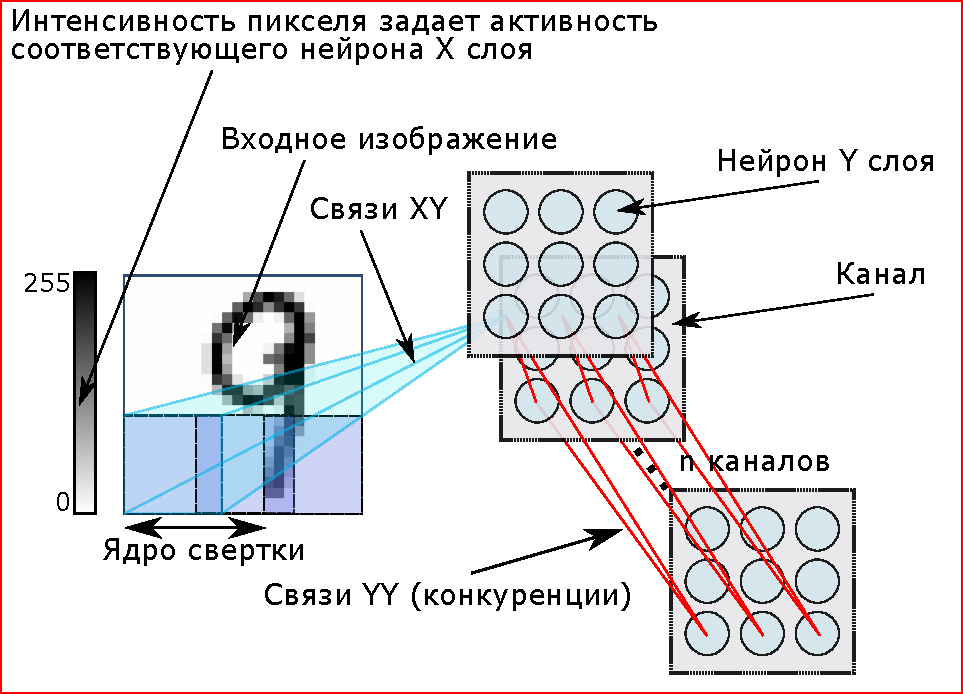
\includegraphics[,
 width=\textwidth,keepaspectratio=true]{LCSNN_ru.pdf} 
    \caption{LCSNN architecture}
\end{figure}

Такие связи имеют отрицательные веса, а значит, негативно влияют на активность. Нейроны, не имеющие общего патча (а значит, реагирующие на разные области изображения), не конкурируют между собой. Связи конкуренции вводятся для улучшения разделения нейронов по выучиваемым признакам. Аналогичная архитектура может быть построена для сетей с использованием сверточных или полносвязных слоев. Исследовались сети с числом $Y$ нейронов $\approx$ 100 --- 900 и параметрами свертки: ширина - 8 или 12, сдвиг - 4. Так как изображения MNIST обрезались до размера 20$\times$20, то число количество нейронов на канал составляло 3 или 4.

В этой работе используется Adaptive Integrate-And-Fire (ALIF) модель нейронов. Динамика потенциала нейрона в этой модели задается уравнением

\begin{equation} \label{eq:alif}
 \tau_v \dv{v(t)}{t} = -v(t) + v_{rest} + I(t) \cdot R \text{,}
\end{equation} где $I(t)$ --- ток, накопившийся в нейроне к моменту времени $t$, $v_{rest}$ --- уровень релаксации, $\tau_v$ --- временная константа симуляции, а $R$ --- размерный коэффициент, численно равный 1.\\ 

Порог активации $v_{thresh}$ у ALIF нейрона не является константой, а немного повышается при каждом спайке, релаксируя затем к своему начальному значению $\theta_o$. Динамика порога активации задается следующими уравнениями:
\begin{equation} 
 v_{thresh} = \theta_0 + \theta(t) \text{,}
\end{equation} где $\theta_0$ --- начальный порог активации, $\theta(t)$ --- адаптивная добавка к порогу активации нейрона после генерации каждого спайка, которая вычисляется из условия\\

\begin{equation}
 \tau_v \dv{\theta(t)}{t} = -\theta(t)
\end{equation}\\

После генерации каждого спайка наступает короткий период рефрактерности, при котором на протяжении времени $t_{refract}$ потенциал нейрона остается на уровне $v_{reset}$. Начальные веса связей задаются случайными числами из равномерного распределения.

\subsection{Обучение прямых связей}
Для уменьшения числа параметров модели изображения обрезаются до размера 20$\times$20 пикселей. Края изображений часто практически пусты, поэтому эта операция практически не влияет на объем информации, доступный сети. Для каждого изображения при помощи распределения Пуассона с математическим ожиданием, пропорциональным интенсивности соответствующего пикселя, генерируются $X$ спайки. Обучение связей $XY$ производится по правилу STDP \cite{STDP}. Это биологически инспирированное правило обучения без учителя \cite{STDP}. При получении пресинаптического импульса (пре-спайка) и испускании пост-спайка вес $w$ связи, по которой пришел пре-спайк, увеличивается на $\Delta w$, где
\begin{equation} 
\Delta w =
 \begin{cases}
 A_+ \cdot e^{- \frac{t_{pre} - t_{post}}{\tau_+}}, t_{pre} - t_{post} > 0\\
 A_- \cdot e^{- \frac{t_{pre} - t_{post}}{\tau_-}}, t_{pre} - t_{post} < 0
 \end{cases}
\end{equation}

Заметим, что

$$
\begin{cases}
 A_{+} > 0\\
 A_{-} < 0
\end{cases}
$$

Таким образом, в процессе обучения у каждого нейрона увеличивается вес связей, по которым пре-спайк систематически приходит непосредственно перед излучением пост-спайка, и наоборот, вес уменьшается у тех связей, для которых такой закономерности не наблюдается. После такого обучения нейрон начинает активнее реагировать на пре-спайки от нейронов, соединенных с ним связями с большими весами, а значит, начинает сам генерировать пост-спайк, если в некотором коротком промежутке времени эти нейроны будут активны одновременно (что означает скоррелированность активностей данных нейронов при выделении некоторого признака). Обратное правило (с противоположными по знаку $A_{+}$ и $A_{-}$) называется правилом anti-STDP \cite{anti-STDP}. В настоящей работе оно используется для обучения связей конкуренции.

После каждой итерации обучения производится нормализация весов --- веса каждого нейрона умножаются на такое число, чтобы их сумма стала равна определенной константе. Это делается для избегания возникновения слишком больших отдельных весов. Значение константы нормализации есть важный гиперпараметр модели, который подбирается для каждой конкретной архитектуры.

\begin{figure}
\centering
\begin{subfigure}{0.45\textwidth}
    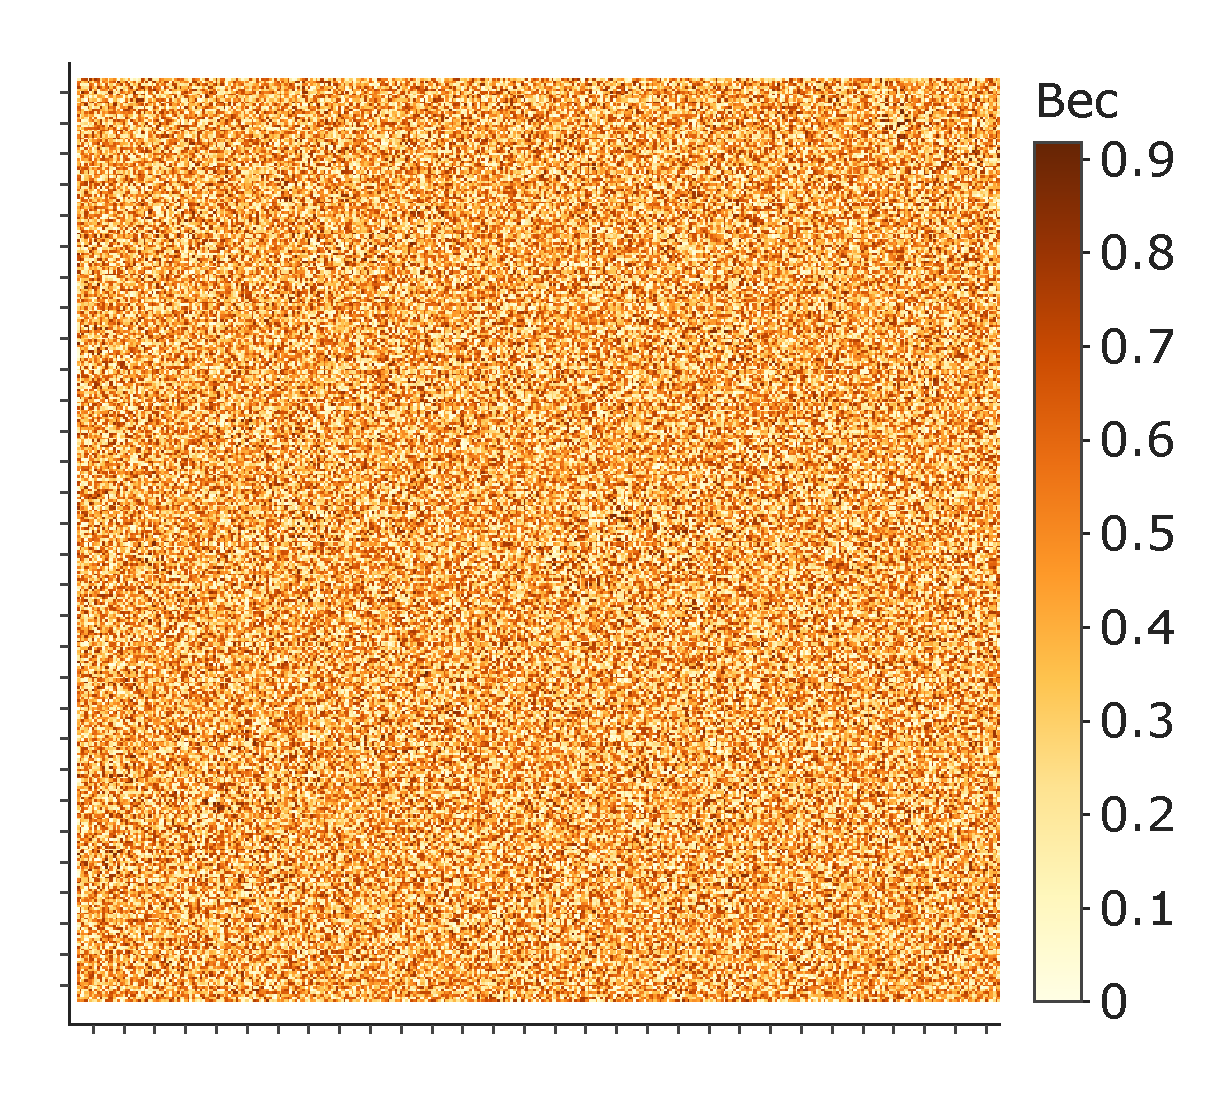
\includegraphics[width=\textwidth,keepaspectratio=true]{weights_XY_untrained_ru.pdf}
    \caption{Перед обучением}
\end{subfigure}
\begin{subfigure}{0.45\textwidth}  \label{weights_XY}
    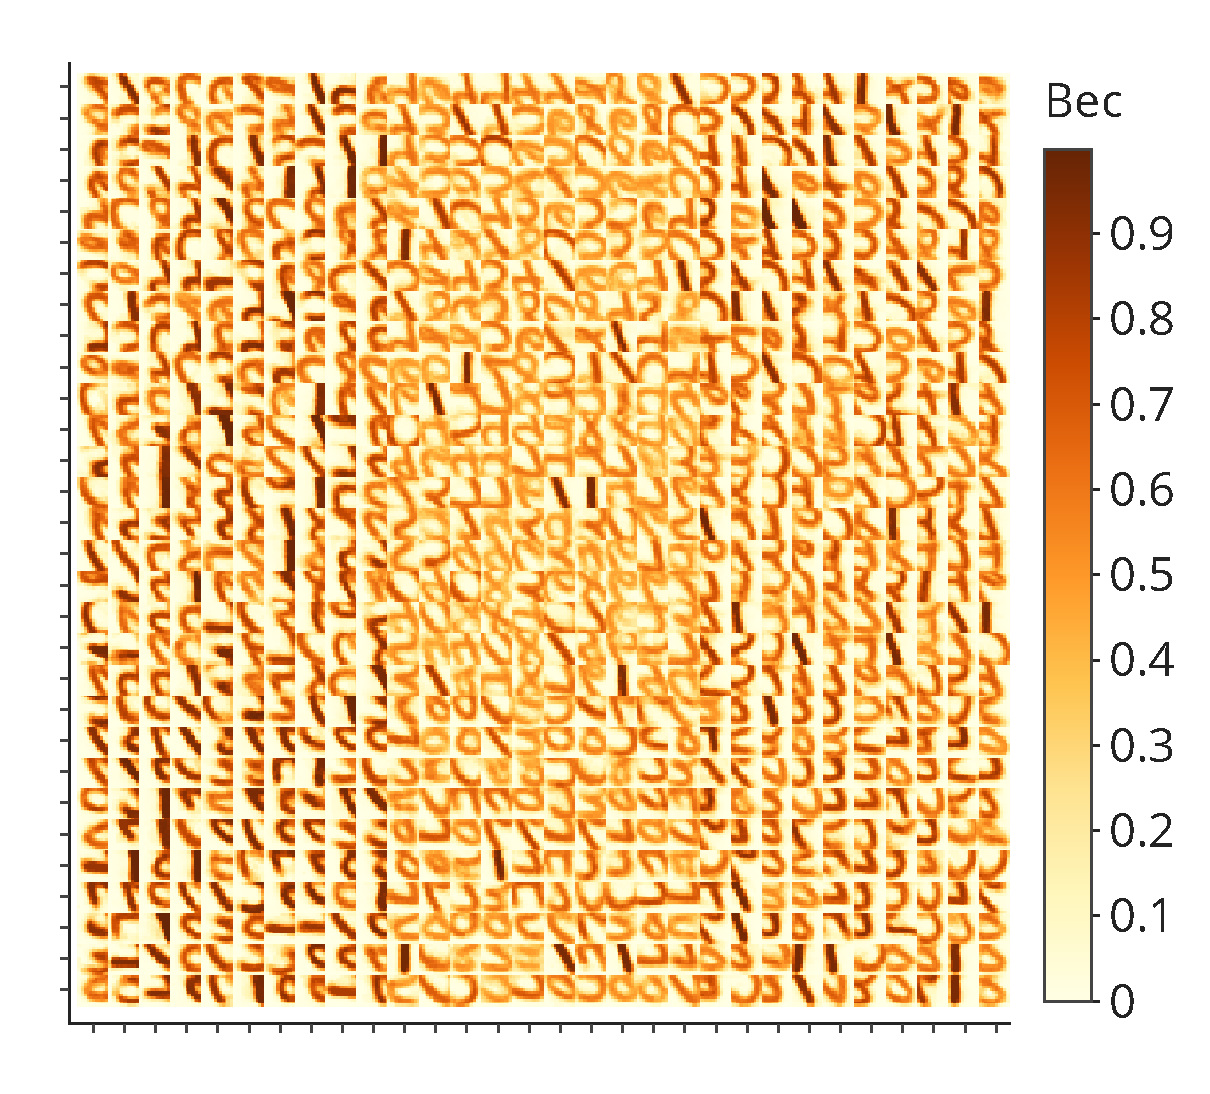
\includegraphics[width=\textwidth,keepaspectratio=true]{weights_XY_ru.pdf}
    \caption{После 10000 итераций обучения}
\end{subfigure}
\caption{Визуализация весов $XY$ связей сети с 900 $Y$ нейронами (по 100 нейронов на каждый из 9 патчей) - матрица 360$\times$360. Веса одного нейрона соответствуют квадрату 12$\times$12. Веса $Y$ нейронов сгруппированы по патчам - левый нижний квадрат 120$\times$120 (10$\times$10 нейронов) соответствует левому нижнему патчу, центральный квадрат соответствует центральному патчу, и так далее. Видно, что после обучения нейроны выучивают некоторые признаки, в которых явно угадываются элементы цифр.}
\end{figure}

\subsection{Интерпретация активности спайковой нейронной сети}

Для интерпретации активности нейронов $Y$ слоя (то есть соотнесения их активности с определенным классом распознаваемых цифр) использовалось несколько методов: голосование патчей, общее голосование нейронов, голосование нейронов с предварительным отбором по спайкам или линейный классификатор. Преимущество первых трех методов заключается в их простоте. Однако, линейный классификатор значительно превосходит их по точности.\\

Для первых трех методов необходимо произвести калибровку голосов нейронов. Каждому нейрону $Y$ слоя ставится в соответствие 10 чисел (голосов) для каждого возможного класса цифр (от 0 до 9). Голос вычисляется как усредненное по различным изображениям число спайков данного нейрона в ответ на демонстрацию сети данной цифры (на протяжении всего времени калибровочной симуляции) ---
$$vote = \frac{\sum_{1}^{n} {\sum_{0}^{t_{max}} s_t}}{n} \text{,}$$
где $s_t$ принимает значение 0 или 1 в зависимости от наличия спайка в данный момент времени, $n$ --- размер калибровочной выборки для каждой цифры ($n = 1000$).

Для всех сетей использовалась калибровка на 10000 примерах из калибровочной выборки, специально отобранной из тестового набора данных, как было отмечено выше. Заметим, что калибровка не является частью обучения сети, так как она входит лишь в алгоритм интерпретации поведения СНС. Эти голоса используются как мера уверенности нейрона в каждом из классов.

\begin{figure}
\centering
\begin{subfigure}{\textwidth}
    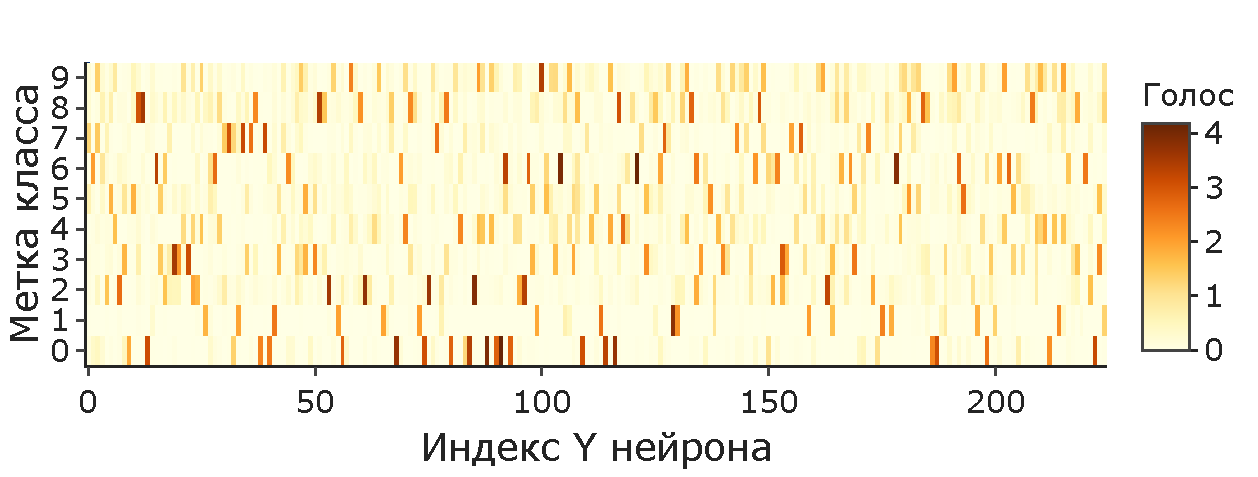
\includegraphics[width=\textwidth,keepaspectratio=true]{votes_ru.pdf}
    \caption{Голоса $Y$ нейронов.}
\end{subfigure}
\begin{subfigure}{\textwidth} 
    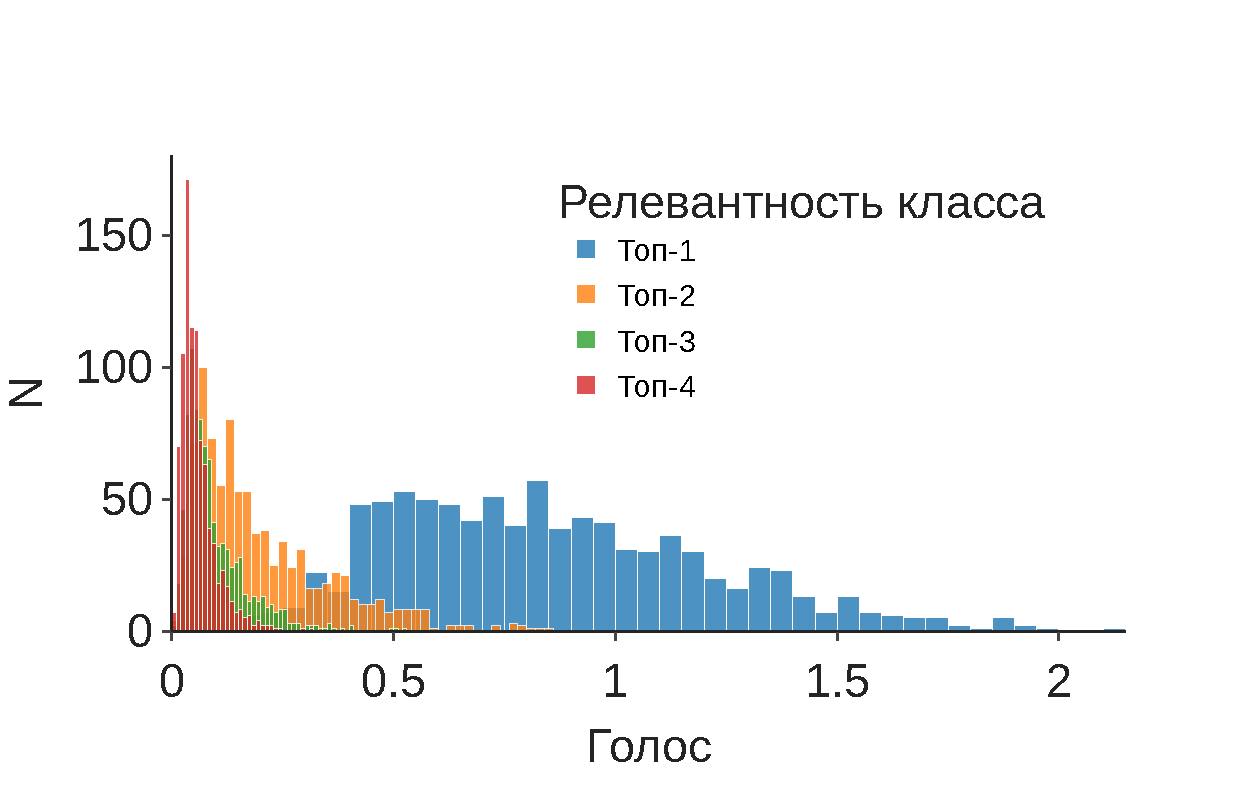
\includegraphics[width=\textwidth,keepaspectratio=true]{votes_distr_4_ru.pdf}
    \caption{Распределения голосов нейронов по четырем наиболее релевантным классам (для каждого нейрона). Видно, что величина голоса (среднее число спайков на класс) сильно падает с уменьшением релевантности.}
\end{subfigure}
\caption{Визуализация голосов нейронов $Y$ слоя сети с 225 $Y$ нейронами. Высокие значения соответствуют большой специализации нейрона на классе. Видно, что практически все нейроны имеют отличное от нуля значение голоса, то есть неактивных нейронов в сети практически нет.}
\end{figure}

Далее результатом будем называть произведение количества спайков нейрона на голос.

При общем голосовании ответом сети считается класс с максимальным результатом среди всех нейронов.

При голосовании патчей для каждого рецептивного поля ищется нейрон с максимальным результатом. Ответом сети считается класс с максимальным результатом среди таких нейронов для всех рецептивных полей.

При отборе по спайкам для каждого рецептивного поля ищется нейрон с максимальным количеством спайков. Ответом сети считается класс с максимальным результатом среди таких нейронов для всех рецептивных полей.

При использовании линейного классификатора на его вход подаются суммы спайков отдельных нейронов $Y$ слоя, а в качестве целевой переменной используются истинные метки классов изображений. Как и в других методах интерпретации активности сети, обучение ведется на калибровочной выборке.

Для оценки работы алгоритма интерпретации используется точность --- отношение количества верно распознанных объектов выборки к размеру тестовой выборки. В этой работе размер тестовой выборки (при измерении точности для отдельных сетей) составляет 10000. 

С целью сравнения алгоритмов интерпретации активности сети были построены кривые обучения для различных алгоритмов интерпретации. Точность измерялась через каждые 250 итераций обучения. Для калибровки алгоритма интерпретации в каждой точке использовалась калибровочная выборка объемом 5000, тогда как для измерения точности – тестовая выборка объемом 1000.

Видно, что через несколько тысяч итераций обучения точность распознавания выходит на плато насыщения, после чего уже не возрастает. Также заметно, что три метода голосования в целом не отличаются по точности, тогда как линейный классификатор значительно превосходит их все. Следует отметить, что точность даже необученной сети может достигать 70\% за счет того, что даже при случайной инициализации весов формируются отдельные нейроны, изначально более склонные к тому или иному классу. Из работы \cite{saunders2019locally} известно, что при достаточно большом числе параметров локально соединенная сеть превосходит сверточную и полносвязную по скорости обучения, так как при каждой итерации обучения обновляется большее число параметров (для каждого рецептивного поля активен минимум один нейрон). В настоящем исследовании не наблюдается такого эффекта, так как представленные кривые обучения построены для недостаточно больших сетей. Интересно, что использование линейного классификатора не повышает точность распознавания для полносвязной сети --- скорее всего, из-за выделения признаков для голосования по всему изображению, в отличие от сверточной и локально связной архитектур.

Линейный классификатор превосходит LCSNN- и CSNN-based алгоритмы голосования по точности, так как является обобщением голосования в том смысле, что при его работе также используется сумма произведений весов (соответствуют голосам) на активности нейронов. Однако, при обучении линейного классификатора представляется возможным использование эффективных алгоритмов оптимизации (в том числе градиентных) его весов, тогда как при голосовании в качестве весов (голосов) используется некая эвристика --- усредненная активность нейронов по классам.

\begin{figure}
\centering
\begin{subfigure}{0.48\textwidth}
    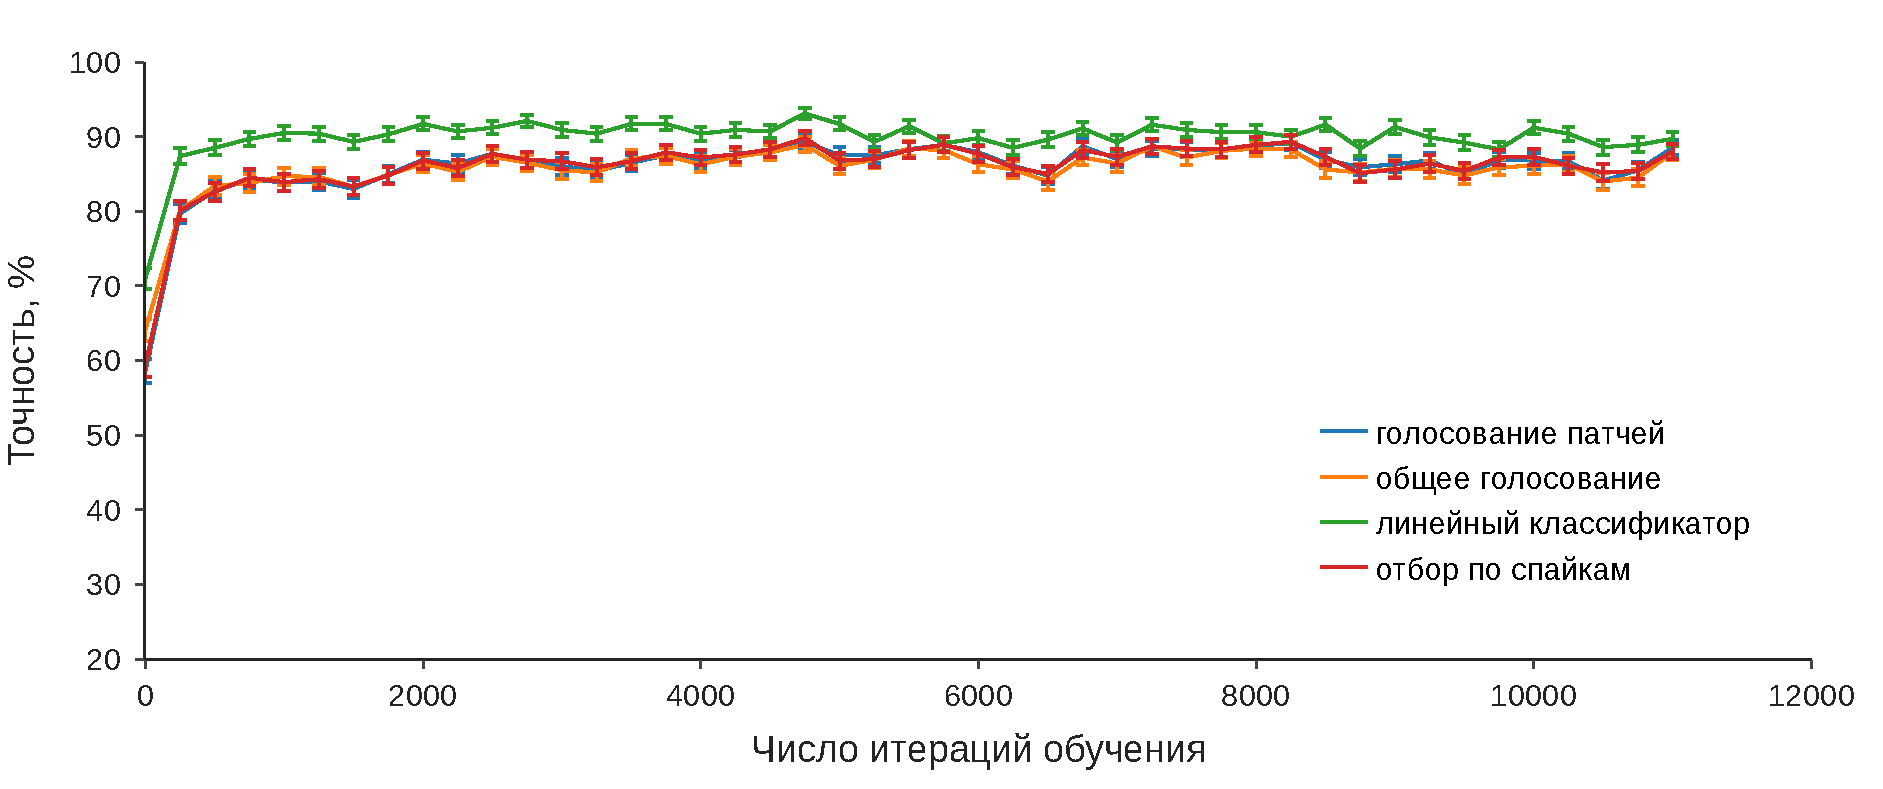
\includegraphics[width=\textwidth,keepaspectratio=true]{LCSNN_learning_rate_ru.pdf}
 \caption{Кривая обучения LCSNN.}
 \label{LCSNN_learning_curve}
\end{subfigure} 
\begin{subfigure}{0.48\textwidth} 
    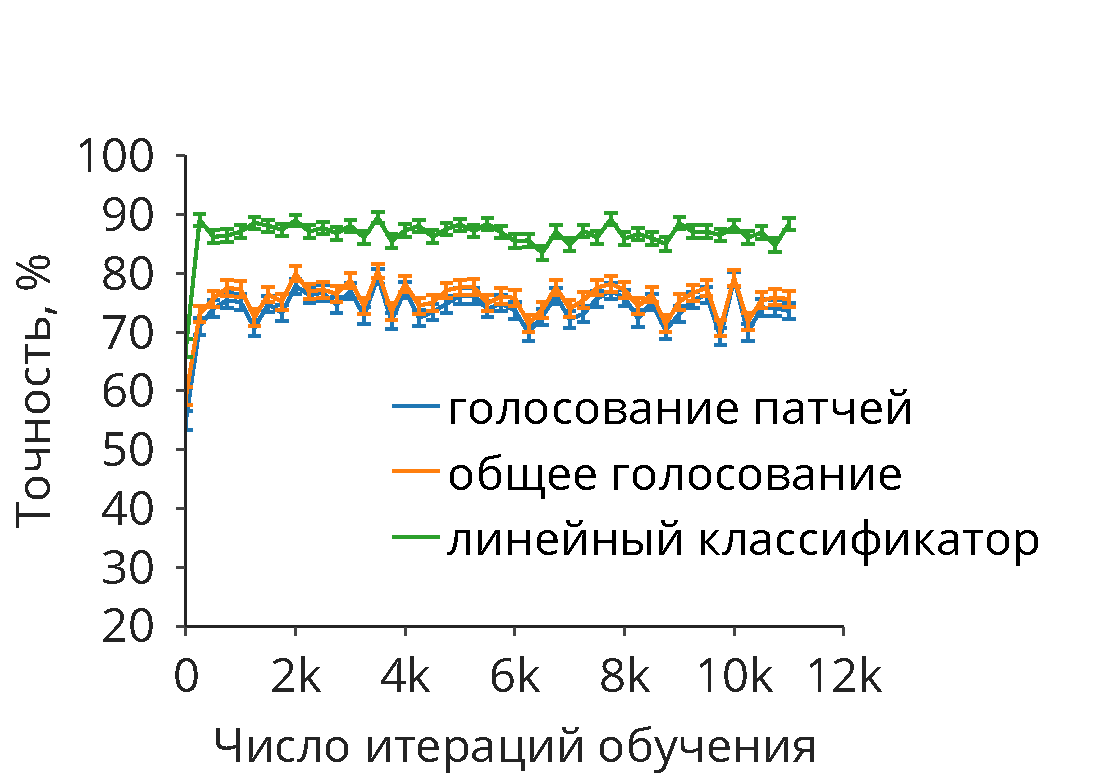
\includegraphics[width=\textwidth,keepaspectratio=true]{CSNN_learning_rate_ru.pdf}
 \caption{Кривая обучения CSNN.}
 \label{CSNN_learning_curve}
\end{subfigure} 
\end{figure}
\begin{figure}\ContinuedFloat
\begin{subfigure}{0.48\textwidth} 
    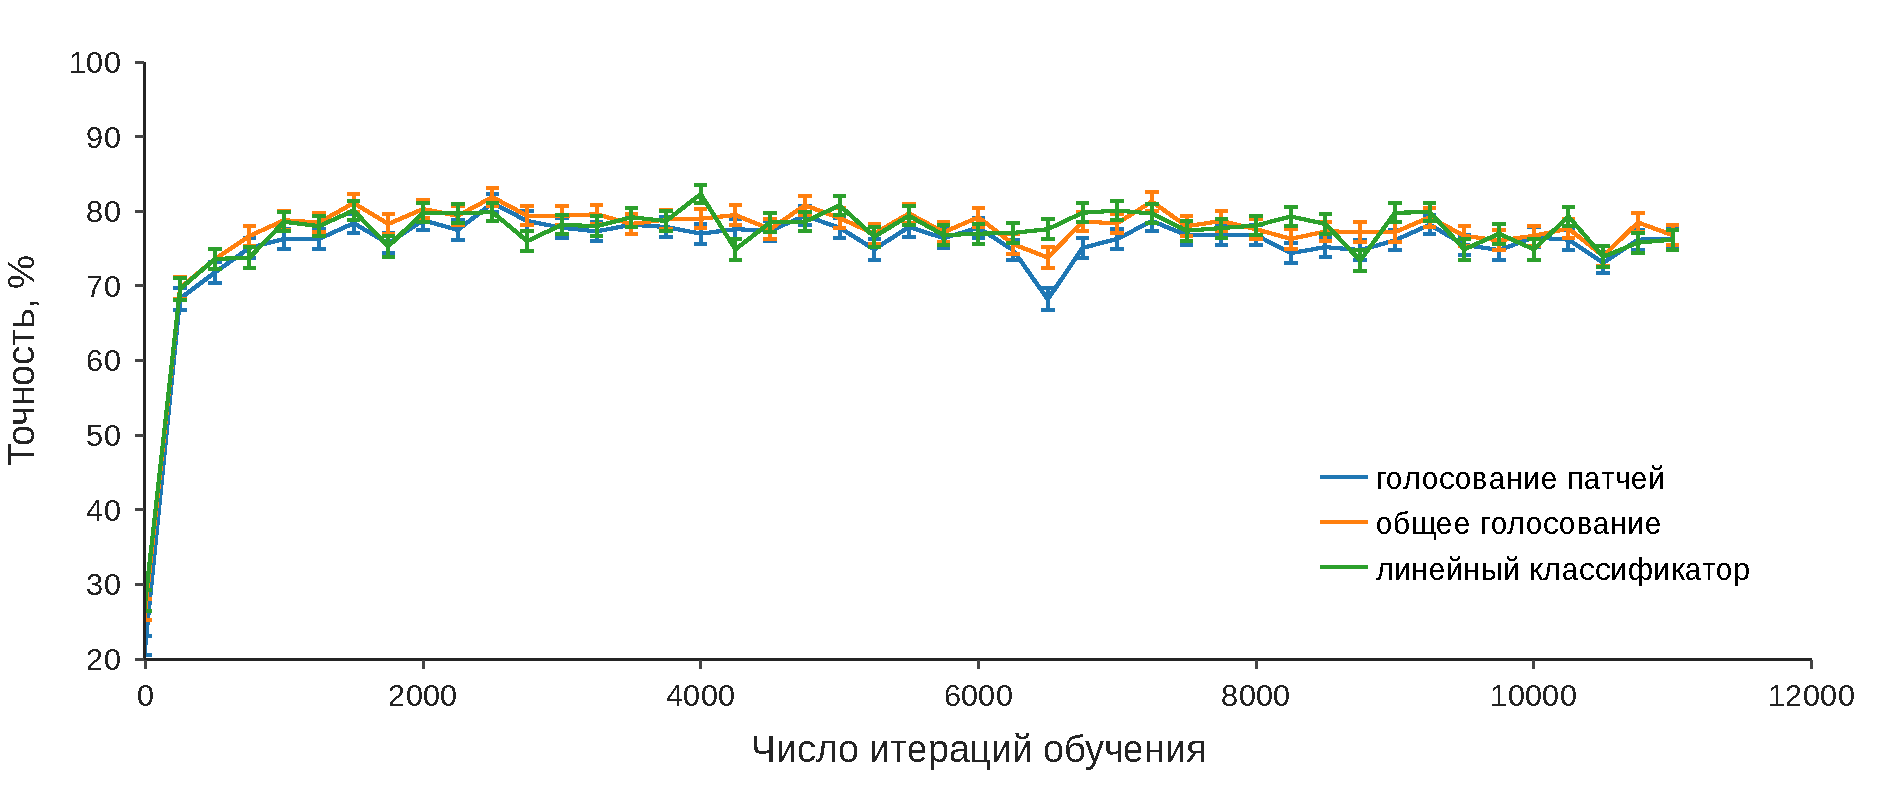
\includegraphics[width=\textwidth,keepaspectratio=true]{FCSNN_learning_rate_ru.pdf}
 \caption{Кривая обучения FCSNN.}
 \label{FCSNN_learning_curve}
\end{subfigure}
\caption{Сравнение кривых обучения различных архитектур спайковых нейронных сетей с конкуренцией: (\ref{LCSNN_learning_curve}) LCSNN, (\ref{CSNN_learning_curve}) CSNN, (\ref{FCSNN_learning_curve}) FCSNN. Приведены результаты для различных алгоритмов интерпретации активности. Отбор по спайкам проверялся только для LCSNN, потому что практически совпадает по результатам с голосованием патчей. В качестве погрешностей нанесены стандартные отклонения. Сети имеют 100 каналов (для FCSNN канал состоит из единственного нейрона), размер свертки для LCSNN составляет 12, а для CSNN --- 8.}
\end{figure}

\subsection{Сравнение эффективности операции свертки и локального рецептивного поля}
Были проведены эксперименты по измерению точности сетей с различными архитектурами. Для сверточных и полносвязных сетей вводились аналогичные LCSNN связи конкуренции. Из-за высоких вычислительных нагрузок не ставилось задачи по нахождению параметров, обеспечивающих максимальную точность для каждой архитектуры. Эти параметры были подобраны приблизительно, однако, судя по результатам отдельных отладочных экспериментов, величина расхождения с оптимальными значениями не превышает 1-2\%. Заметим, что при использовании линейного классификатора в качестве алгоритма интерпретации удалось достигнуть 95\% точности для локально соединенной сети из 1000 каналов с размером ядра 12.


\begin{table}
 \caption{Результаты сравнения различных архитектур спайковых нейронных сетей. Для каждой конфигурации точность измерялась $N=5$ раз. В таблице указаны среднее арифметическое значение точности и его стандартное отклонение. <<Ядро>> соответсвует числу $k$ в размере свертки $k\times k$.}
\begin{center}
\begin{adjustwidth}{-1cm}{}
\begin{tabular}{|l|l|l|l|l|l|p{2.2cm}|p{2.2cm}|}
\hline
&\multicolumn{5}{c|}{Конфигурация} & \multicolumn{2}{c|}{Точность, \%}\\
\hline
N & Архитектура & Каналы & Ядро & Параметры & $Y$ нейроны & {Метод \footnotemark[1]} & {Метод \footnotemark[2]} \\
\hline\hline
{\textbf{1}} & {\textbf{LCSNN}} & {\textbf{1000}} & {\textbf{12}} & {\textbf{10287000}} & {\textbf{9000}} & {$\mathbf{92.3 \pm 0.7}$} & {$\mathbf{95.1 \pm 0.5}$}\\
\hline
2 & {LCSNN} & {100} & {12} & {218700} & {900} & {$87.5 \pm 0.9$} & {$91.5 \pm 0.6$}\\
\hline
3 & {LCSNN} & {100} & {8} & {260800} & {1600} & {$82.9 \pm 0.6$} & {$88.1 \pm 0.7$}\\
\hline
{\textbf{4}} & {\textbf{LCSNN\footnotemark[3]}} & {\textbf{25}} & {\textbf{12}} & {\textbf{37800}} & {\textbf{225}} & {$\mathbf{82.3 \pm 1.0}$} & {$\mathbf{88.2 \pm 0.6}$}\\
\hline
5 & {LCSNN} & {25} & {12} & {37800} & {225} & {$80.1 \pm 1.0$} & {$85.5 \pm 0.8$}\\
\hline
6 & {LCSNN} & {25} & {8} & {35200} & {400} & {$73.6 \pm 1.0$} & {$80.3 \pm 0.7$}\\
\hline\hline
7 & {CSNN} & {169} & {12} & {279864} & {1521} & {$79.2 \pm 1.6$} & {$85.7 \pm 1.4$}\\
\hline
8 & {CSNN} & {81} & {12} & {69984} & {729} & {$77.2 \pm 1.7$} & {$83.1 \pm 1.2$}\\
\hline
9 & {CSNN} & {100} & {8} & {164800} & {1600} & {$77.4 \pm 1.9$} & {$82.1 \pm 1.3$}\\
\hline
10 & {CSNN} & {25} & {12} & {9000} & {225} & {$65.8 \pm 0.7$} & {$77.1 \pm 0.6$}\\
\hline
11 & {CSNN} & {25} & {8} & {11200} & {400} & {$63.1 \pm 1.2$} & {$75.8 \pm 0.5$}\\
\hline\hline
12 & {FCSNN} & {100} & {20} & {49900} & {100} & {$81.4 \pm 0.9$} & {$82.1 \pm 0.8$}\\
\hline
\end{tabular}
\end{adjustwidth}
\end{center}
 \label{results}
\end{table}

\footnotetext[1]{Лучший алгоритм голосования}
\footnotetext[2]{Линейный классификатор}
\footnotetext[3]{Сеть с обучением связей конкуренции}

Видно (№2 и №7 в таблице \ref{results}), что локально соединенная сеть превосходит сверточную сеть по точности даже при чуть превышающем числе параметров последней. Также, можно заметить, что не следует использовать слишком малый размер ядра свертки. Это приводит к выучиванию менее существенных признаков. Действительно, в традиционном машинном обучении на основе ИНН используются либо неглубокие сети с большими ядрами свертки, либо глубокие модели, но, наоборот, с маленькими ядрами свертки.

Следует отметить, что SNN могут достигать значительно больших точностей распознавания на MNIST. Для этого можно использовать: (i) cети с существенно большим числом весовых параметров (например, с увеличенным числом каналов); (ii) более глубокие сети (с большим количеством слоев); (iii) более эффективные на сегодня алгоритмы обучения (например, обучение с учителем или с использованием контрастивной функции потерь \cite{contrastive_loss}). В то же время, достижение максимально возможной точности не являлось целью настоящего исследования, адресованного, в первую очередь, сравнению различных архитектур SNN.

\begin{table}
 \caption{Результаты других исследований спайковых нейронных сетей. Во всех используется датасет MNIST.}
\begin{center}
\begin{tabular}{|l|p{4cm}|p{7cm}|l|l|}
\hline
Статья & Архитектура & Обучение & Точность, \% \\
\hline\hline
{Эта работа} & {Локальная + конкуренция} & {Без учителя} & {$95.1 \pm 0.5$}\\
\hline\hline
{\cite{saunders2019locally}} & {Локальная + конкуренция} & {Без учителя} & {$95.07 \pm 0.63$}\\
\hline
{\cite{mnist2}} & {Полносвязная + конкуренция} & {Без учителя} & {95}\\
\hline
{\cite{MaxActiv1}} & {Полносвязная + конкуренция} & {С учителем / с частичным привлечением учителя} & {95.4 / 72.1}\\
\hline
{\cite{conv1}} & {Сверточная} & {С частичным привлечением учителя} & {$96.95 \pm 0.08$}\\
\hline
{\cite{conv2}} & {Сверточная} & {С частичным привлечением учителя} & {$99.28 \pm 0.10$}\\
\hline
{\cite{conv3}} & {Сверточная} & {С частичным привлечением учителя} & {$97.20 \pm 0.07$}\\
\hline
\end{tabular}
\end{center}
\end{table}

Результат, полученный в настоящей работе, практически соответствует результату из \cite{saunders2019locally}. Заметим, что при помощи признаков, обученных без учителя достигаются результаты, лишь немногим уступающие результатам, полученным при помощи обучения с учителем. При этом лучшая локально соединенная сеть с конкуренцией локальных рецептивных полей из этой работы имеет $10^7$ связей (из них связей прямого распространения --- $1 \cdot 10^6$, связей конкуренции --- $9 \cdot 10^6$), по сравнению с $4.6 \cdot 10^7$ (из них связей прямого распространения --- $0.5 \cdot 10^7$, связей конкуренции --- $4.1 \cdot 10^7$) у полносвязной сети с конкуренцией из \cite{mnist2}. К тому же, обучение сети из \cite{mnist2} велось в течение $1 \cdot 10^6$ итераций, тогда как в этой работе число итераций обучения не превосходит 5000.

\section{Обучение связей конкуренции}
Ингибирующие связи $YY$ существенно влияют на обучение связей прямого распространения сигнала $XY$. Большие по модулю значения весов конкуренции способствуют большей вариативности и специализации в обучении $Y$ нейронов, так как для каждого рецептивного поля одновременно активными не могут быть нейроны, имеющие схожие веса $XY$ (Рис. \ref{fig:high_comp}). Наоборот, малые по модулю веса конкуренции не позволяют нейронам эффективно специализироваться (Рис. \ref{fig:high_comp}).

\begin{figure}
\centering
\begin{subfigure}{0.45\textwidth}
    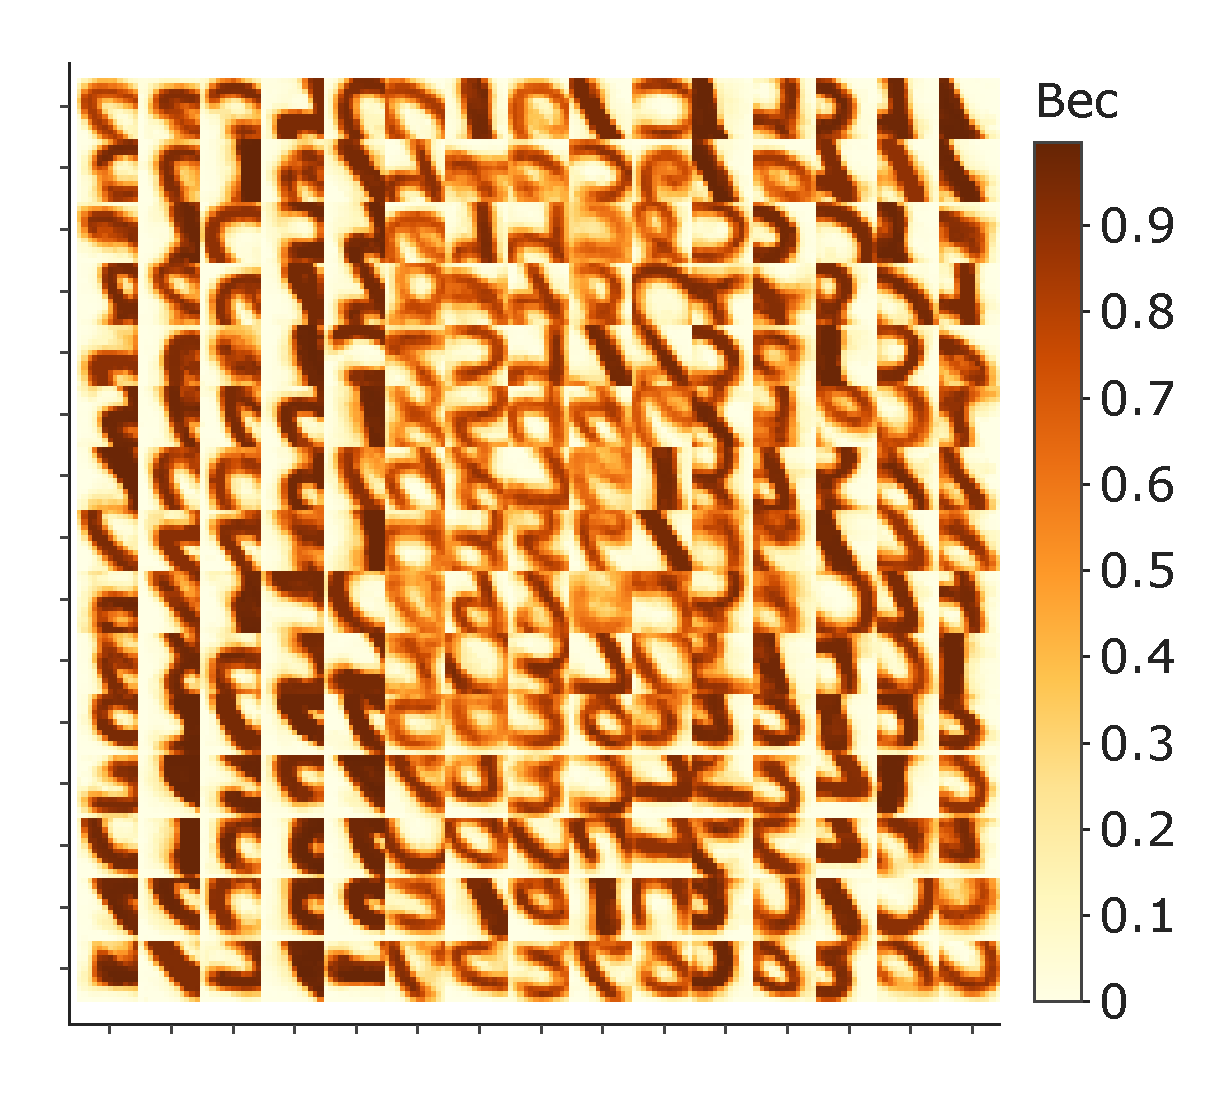
\includegraphics[width=\textwidth,keepaspectratio=true]{weights_XY_good_ru.pdf}
    \caption{Высоко специализированные веса, вес конкуренции равен --100.}
    \label{fig:high_comp}
\end{subfigure}
\begin{subfigure}{0.45\textwidth}
    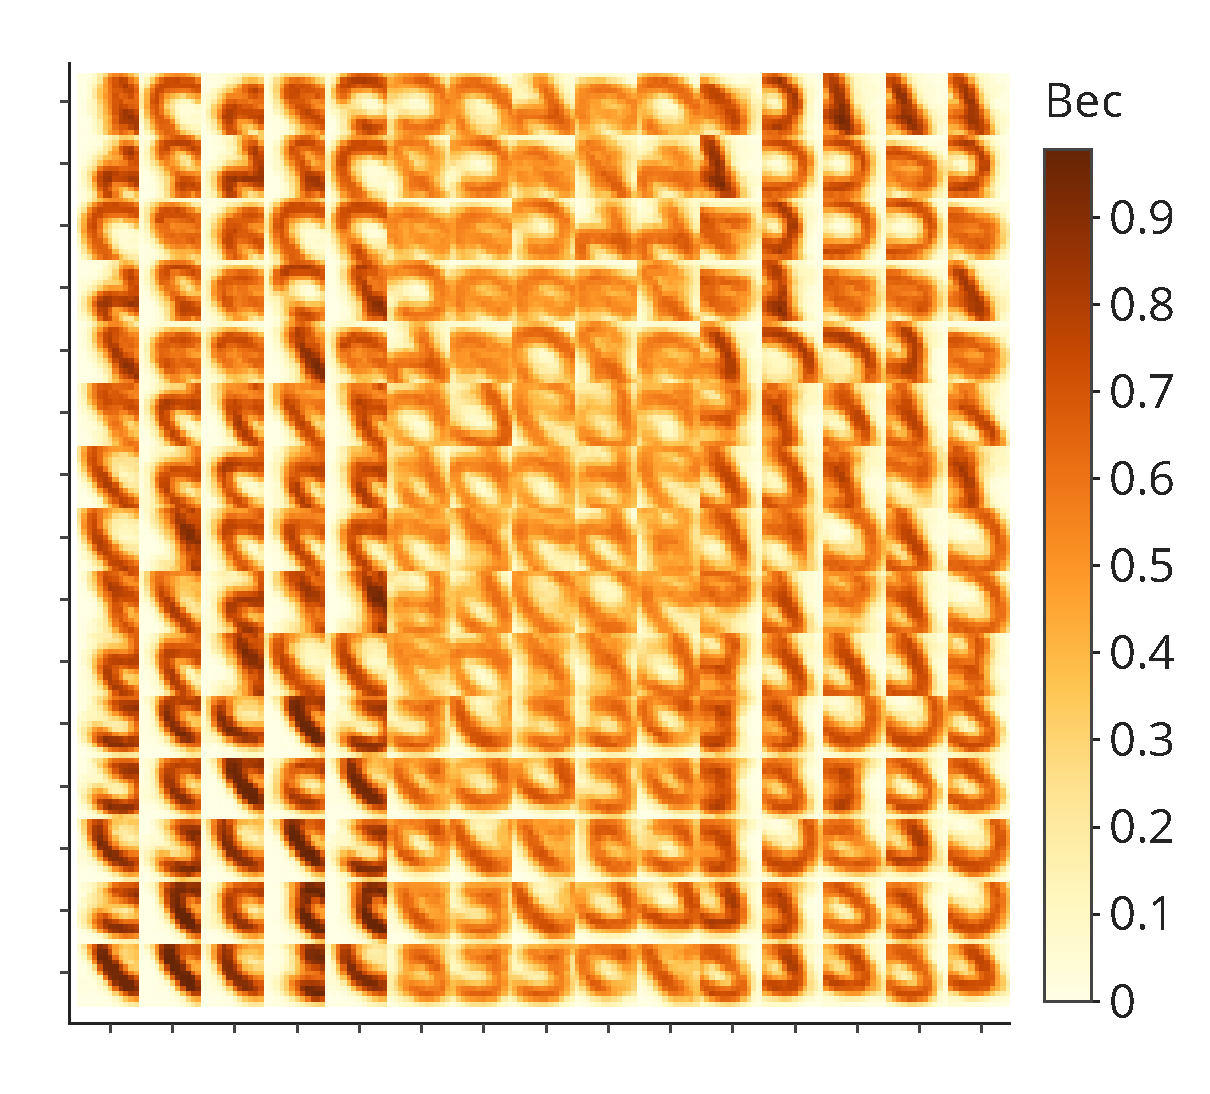
\includegraphics[width=\textwidth,keepaspectratio=true]{weights_XY_bad_ru.pdf}
    \caption{Слабо специализированные веса,\\ вес конкуренции равен --10.}
    \label{fig:low_comp}
\end{subfigure}
\caption{Влияние конкуренции на обучение связей $XY$.}
\label{competition-training-importance}
\end{figure}

Все SNN, о которых шла речь в настоящей работе до этого момента, имели фиксированные веса конкуренции. В связи с этим, возникает вопрос, как влияет на точность сети обучение весов конкуренции. Для ответа на поставленный вопрос с целью обновления связей $YY$ было выбрано правило anti-STDP (правило, противоположное по знакам $A_{+}$ и $A_{-}$ в стандартном STDP). При варьировании значений параметров этого правила были получены различные распределения весов конкуренции. Начальные значения весов конкуренции задавались из равномерного распределения от 0 до некоторого числа, которое в дальнешем будем называть начальным весом конкуренции. Эксперименты проводились с LCSNN.

\begin{table}
 \caption{Параметры anti-STDP}
\begin{center}
\begin{tabular}{|l|l|l|l|l|}
\hline
Рисунок & {$\tau_{+}$, мс} & {$\tau_{-}$, мс} & {$A_{+}$} & {$A_{-}$} \\
\hline
\ref{fig:worst_competition_distribution} & 14.7 & 14.2 & -0.5 & -1.5 \\
\hline
\ref{fig:medium_bad_competition_distribution} & 5.4 & 15.1 & -1.2 & -0.6 \\
\hline
\ref{fig:medium_good_competition_distribution} & 17.6 & 24.5 & -1.9 & -1.6 \\
\hline
\ref{fig:best_competition_XY} & 17.7 & 16.5 & -0.1 & -1.6\\
\hline
\end{tabular}
\end{center}
\end{table}

\begin{figure}
\centering
\begin{subfigure}{0.45\textwidth}
    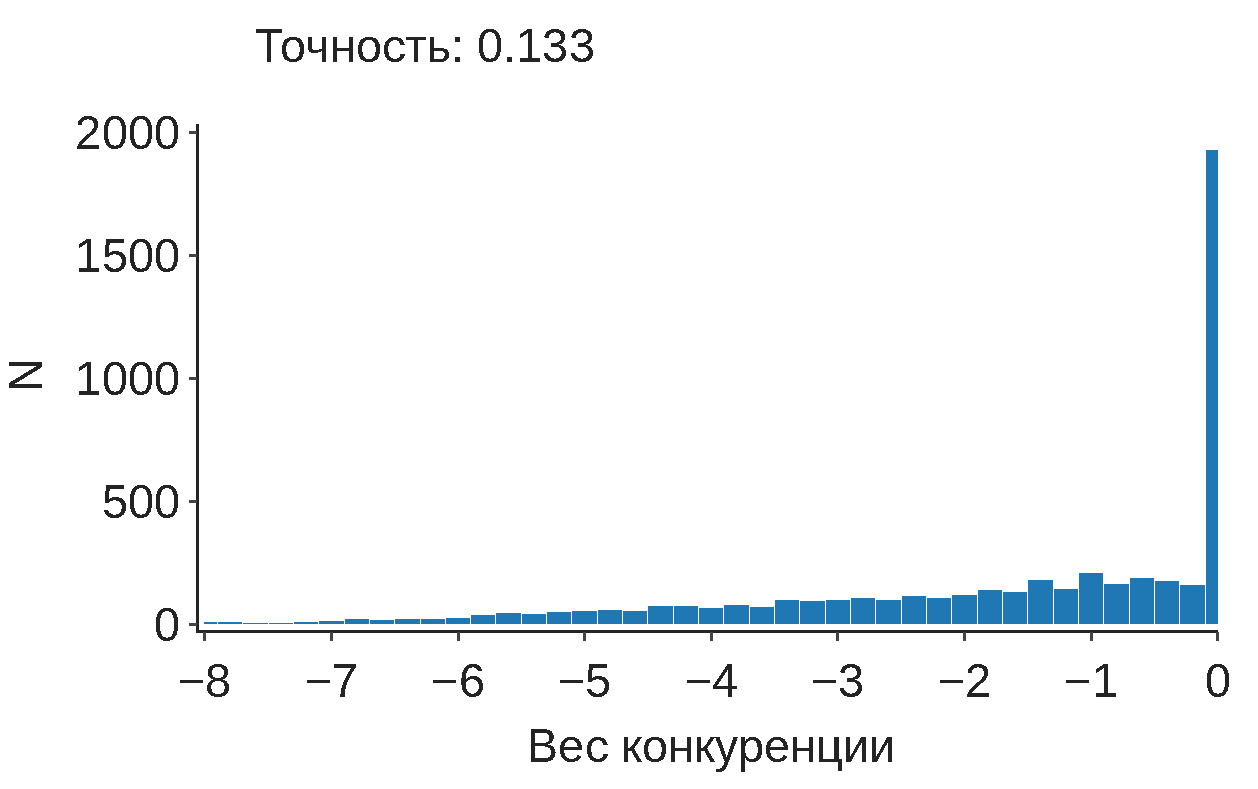
\includegraphics[width=\textwidth,keepaspectratio=true]{competition_distribution_worst_ru.pdf}
    \caption{Очень слабая конкуренция}
\end{subfigure}
\begin{subfigure}{0.45\textwidth}
    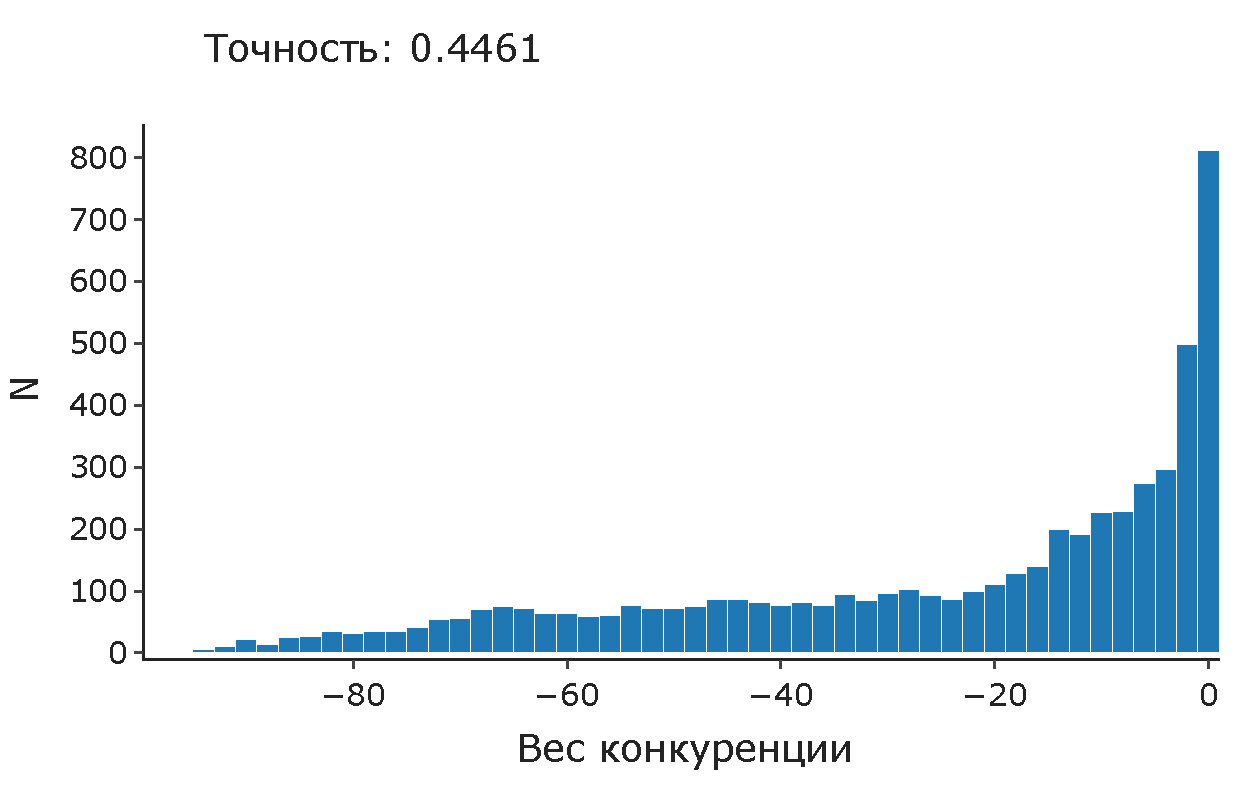
\includegraphics[width=\textwidth,keepaspectratio=true]{competition_distribution_medium_bad_ru.pdf}
    \caption{Слабая конкуренция}
\end{subfigure}
\\
\begin{subfigure}{0.45\textwidth}
    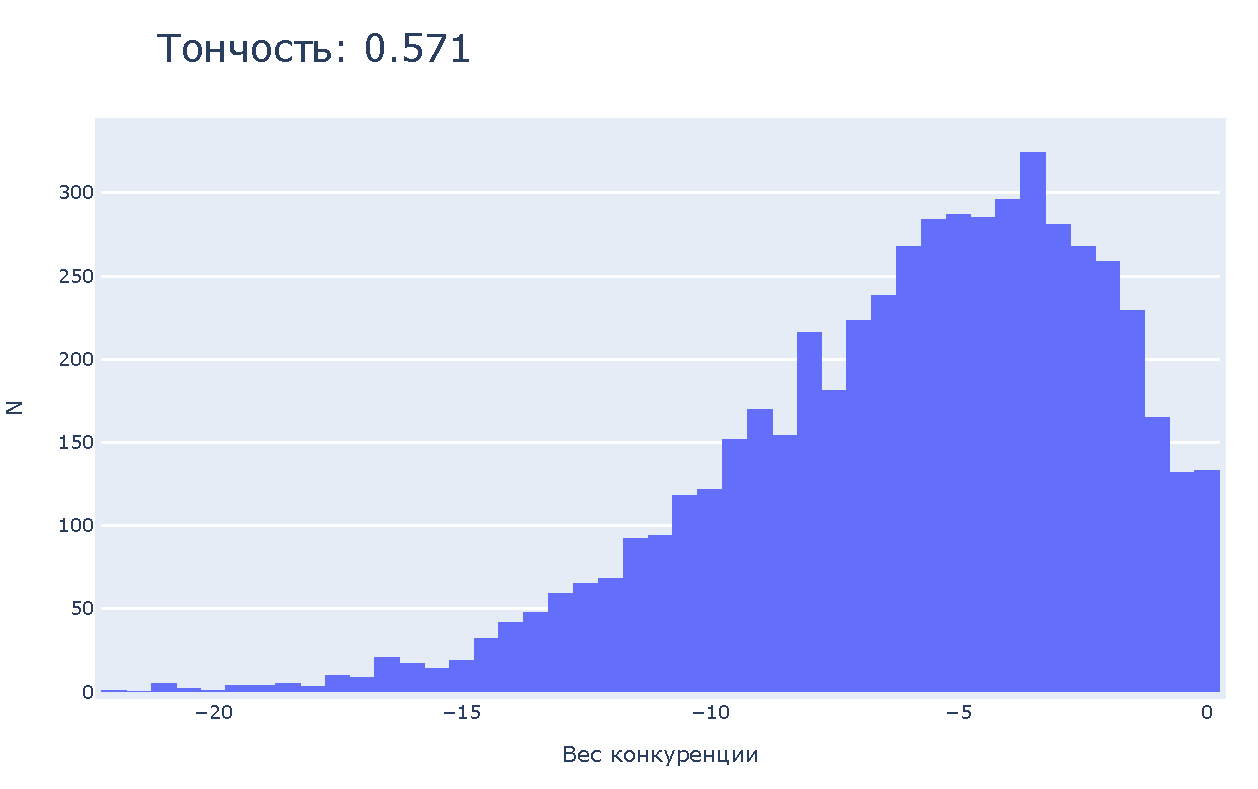
\includegraphics[width=\textwidth,keepaspectratio=true]{competition_distribution_medium_good_ru.pdf}
    \caption{Средняя конкуренция} 
\end{subfigure}
\begin{subfigure}{0.45\textwidth}
    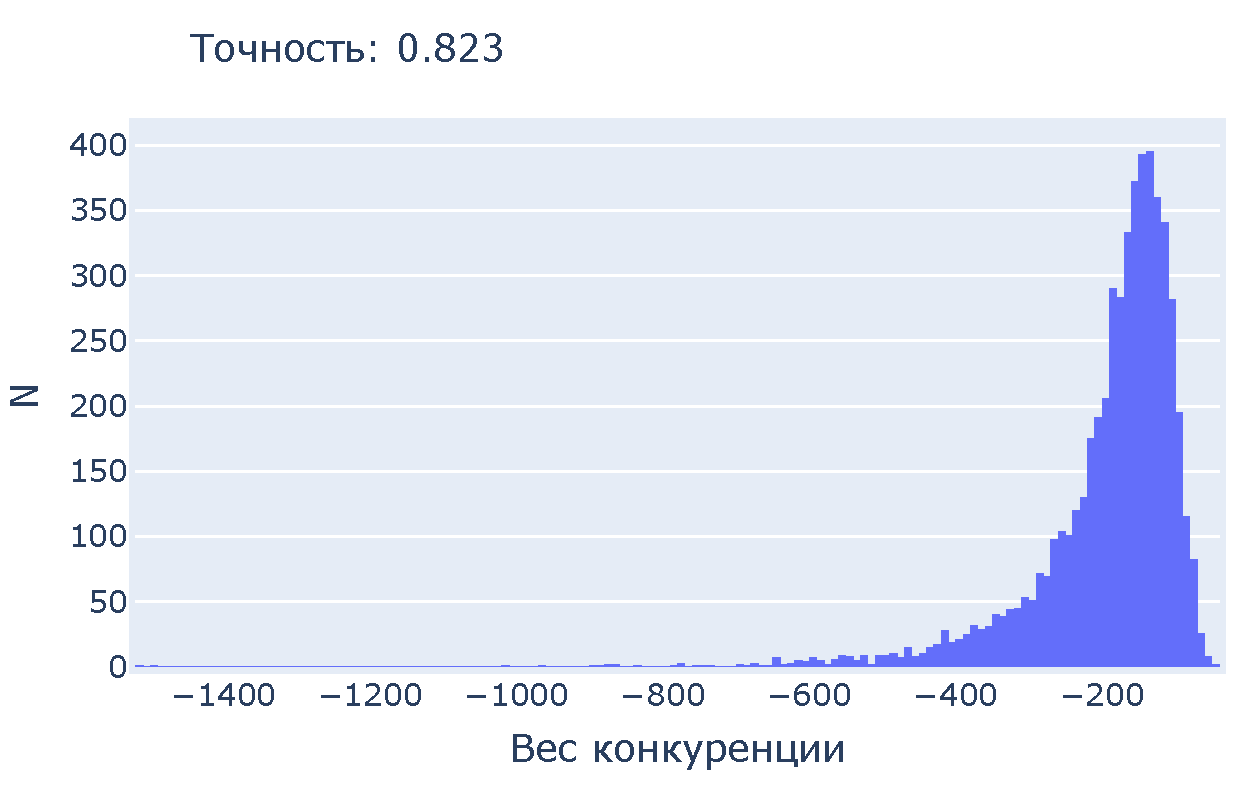
\includegraphics[width=\textwidth,keepaspectratio=true]{competition_distribution_best_ru.pdf}
    \caption{Сильная конкуренция}
    \label{fig:best_competition}
\end{subfigure}
\caption{Различные распределения весов конкуренции}
\label{fig:competition_distributions}
\end{figure}

Видно, что точность сети повышается при смещении распределения весов конкуренции в сторону больших по модулю отрицательных значений. Заметим опять, что целью являлось не нахождение параметров сети, обеспечивающих максимальную точность, а исследование влияния способности обучения конкуренции на точность сети с заданной конфигурацией остальных параметров.

Примечательно, что не все связи $YY$ получают большие по модулю значения (Рис. \ref{fig:best_competition}). Это объясняется тем, что нейроны, специализирующиеся на существенно разных признаках, не нуждаются в конкуренции, так как они не проявляют высокую активность одновременно.

\begin{figure}
\centering
\begin{subfigure}{0.45\textwidth} 
    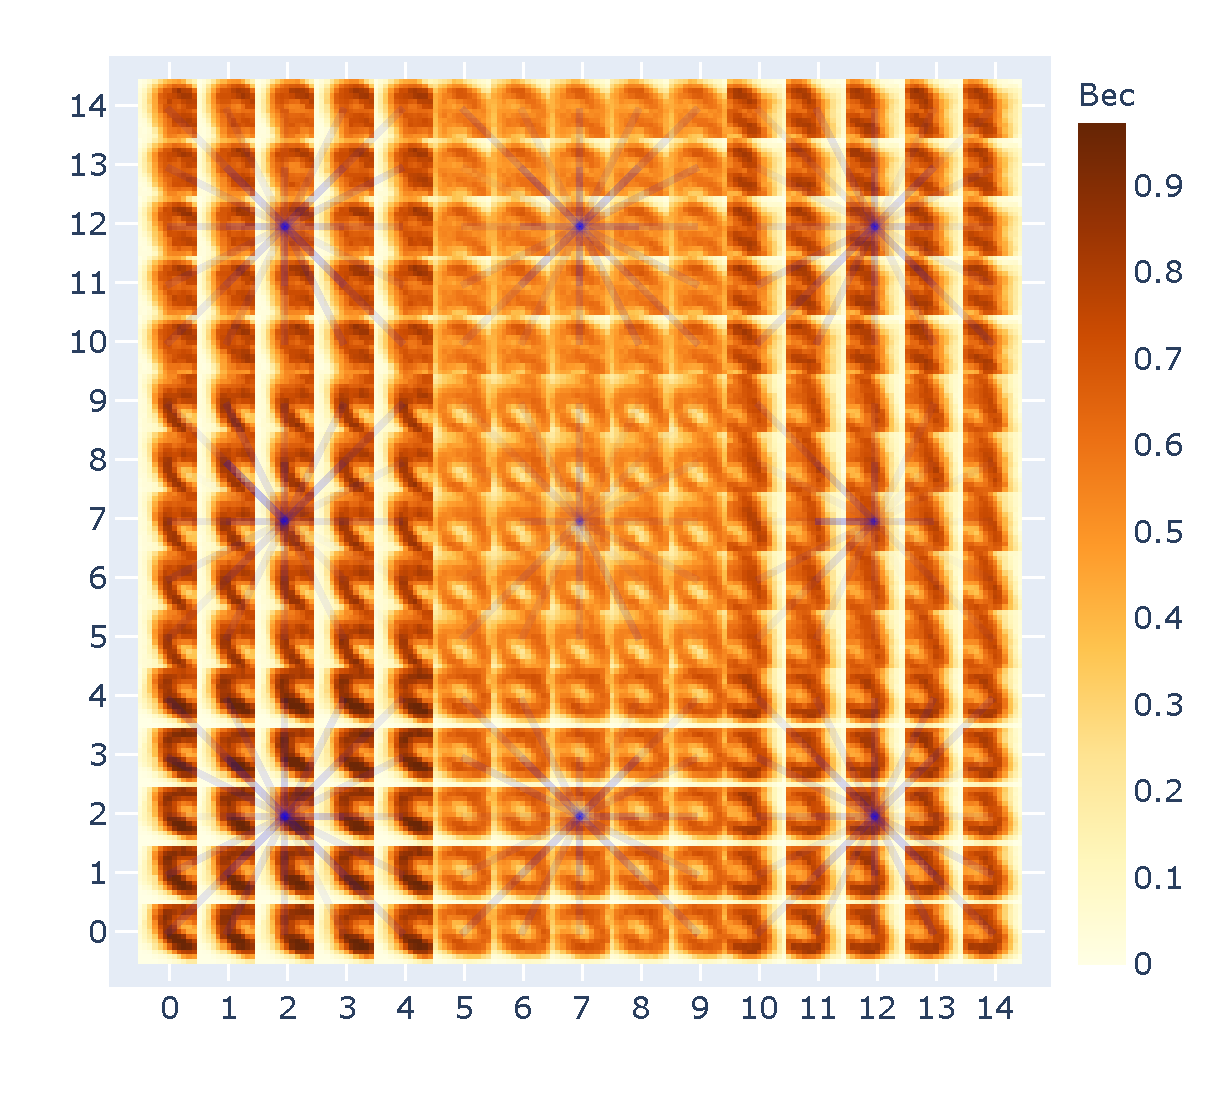
\includegraphics[width=\textwidth,keepaspectratio=true]{competition_on_XY_worst_ru.pdf}
    \caption{Очень слабая конкуренция}
    \label{fig:worst_competition_distribution}
\end{subfigure}
\begin{subfigure}{0.45\textwidth}
    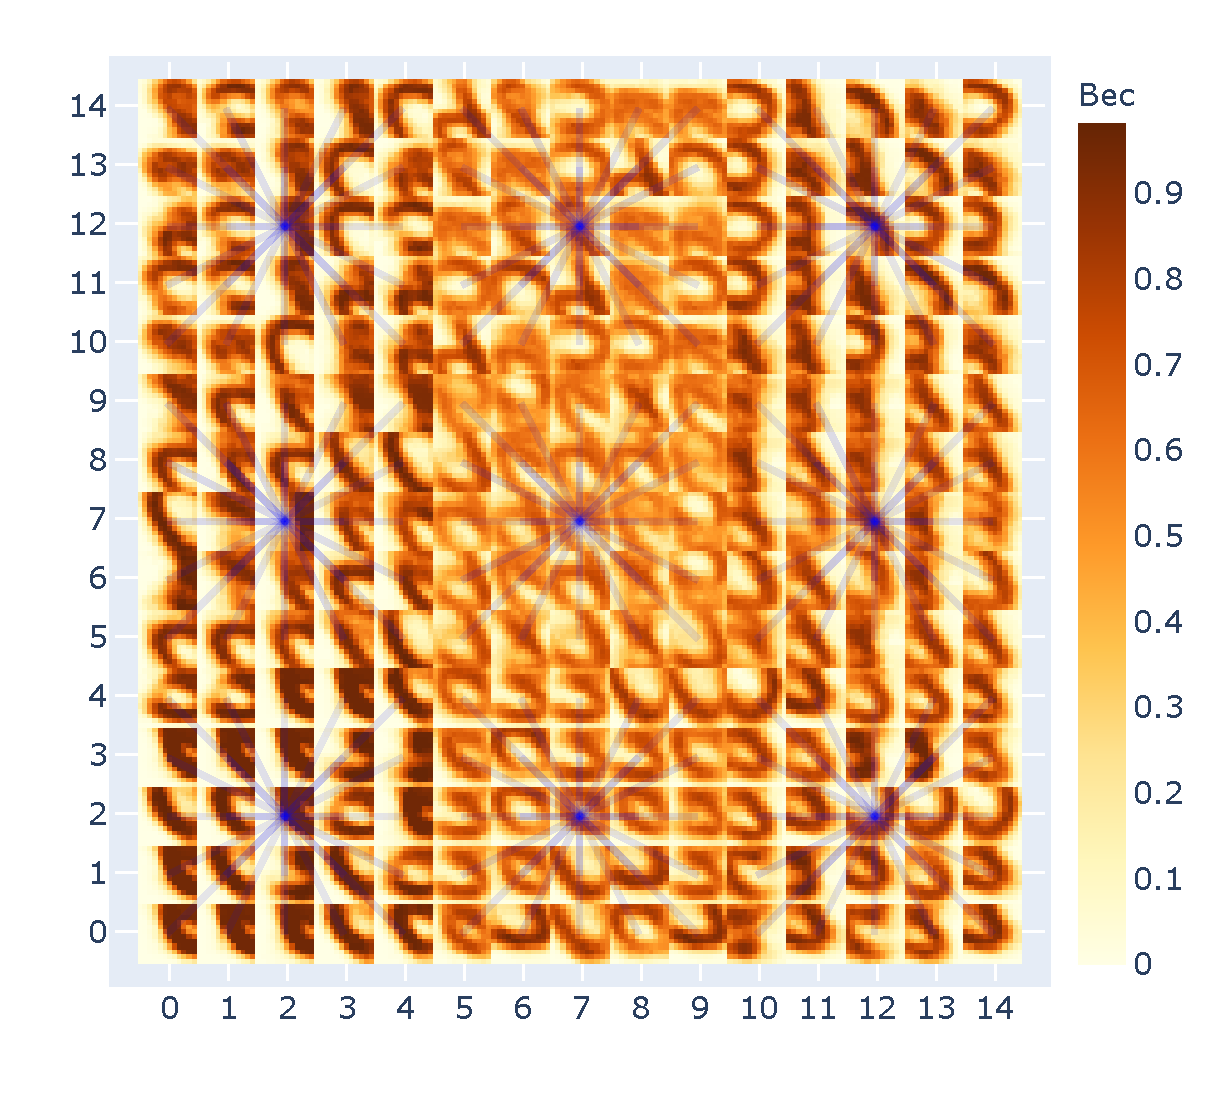
\includegraphics[width=\textwidth,keepaspectratio=true]{competition_on_XY_medium_bad_ru.pdf}
    \caption{Слабая конкуренция}
    \label{fig:medium_bad_competition_distribution}
\end{subfigure}
\\
\begin{subfigure}{0.45\textwidth}
    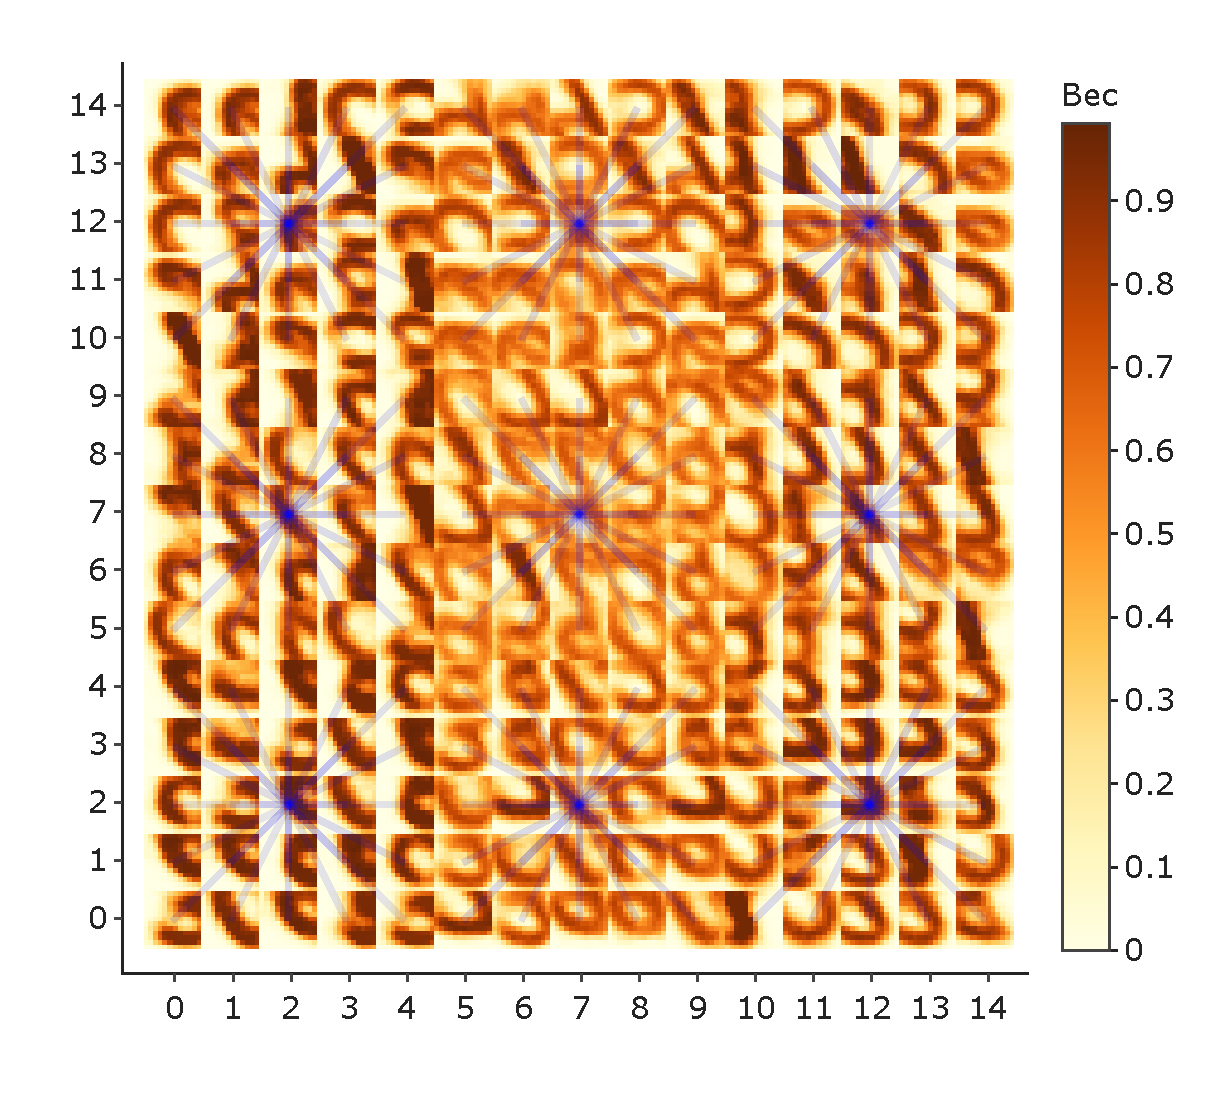
\includegraphics[width=\textwidth,keepaspectratio=true]{competition_on_XY_medium_good_ru.pdf}
    \caption{Средняя конкуренция}
    \label{fig:medium_good_competition_distribution}
\end{subfigure}
\begin{subfigure}{0.45\textwidth} 
    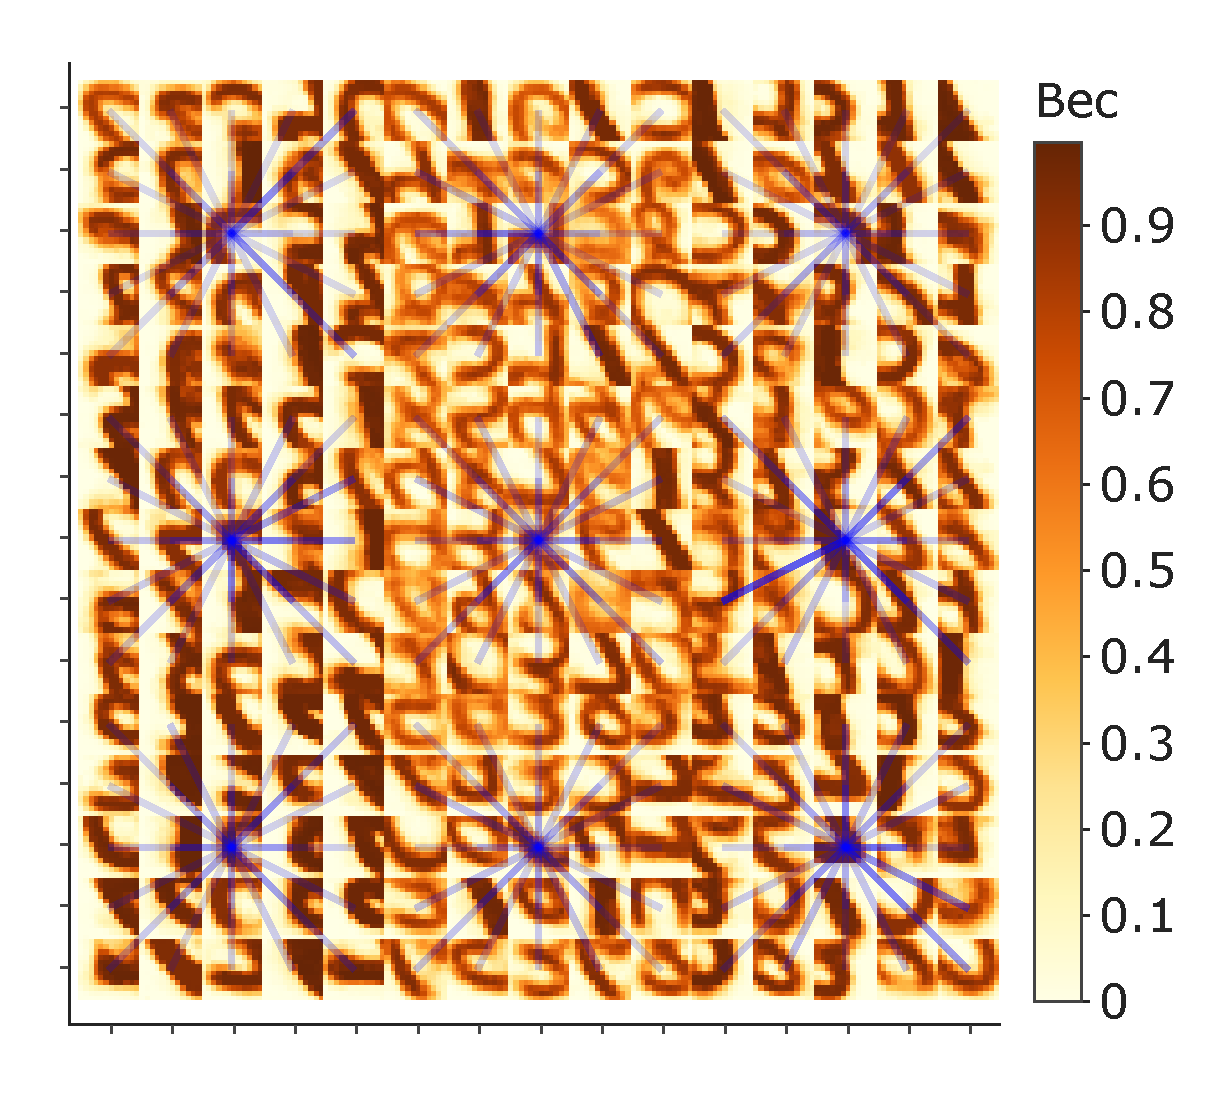
\includegraphics[width=\textwidth,keepaspectratio=true]{competition_on_XY_best_ru.pdf}
    \caption{Сильная конкуренция}
    \label{fig:best_competition_XY}
\end{subfigure}
\caption{Визуализация весов конкуренции поверх весов $XY$. Изображения соответствуют весам сетей с рисунка \ref{fig:competition_distributions}. Изображены только веса конкуренции для одного нейрона в каждом рецептивном поле для избегания загромождения визуализации. Насыщенный синий цвет соответствует большим по модулю весам конкуренции (используется среднее арифметическое между весами $W_{ij}$ и $W_{ji}$). Видно, что похожие признаки сильнее конкурируют между собой, чем различные.}
\end{figure} 

Обучение конкуренции производилось только на сетях из 25 каналов (225 нейронов), так как его моделирование требует больших вычислительных ресурсов.

В ходе оптимизации моделей была измерена точность большого количества LCSNN с различными конфигурациями гиперпараметров (Рис. \ref{fig:hyperparams}). Видно, что конфигурации с высокими точностями (темные ломаные) локализуются определенным образом - дописать

\begin{figure}
\begin{center}
 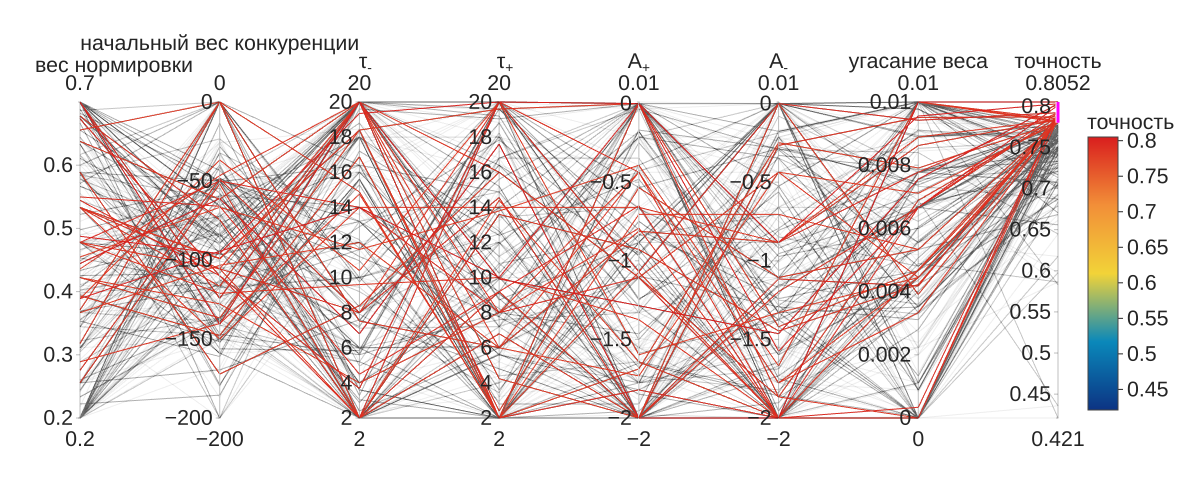
\includegraphics[,
 width=\textwidth,keepaspectratio=true]{hyperparams_ru.png}
 
\caption{Визуализация достигаемой точности распознавания LCSNN при использовании различных комбинаций параметров в пространстве гиперпараметров. Параметры <<вес нормировки>>, <<начальный вес конкренции>> и <<угасание веса>> отвечают за значения весов, а следующие два являются комбинациями параметров anti-STDP. На последней оси указана точность сети с конфигурацией, соответствующих точкам пересечения ломаной осей гиперпараметров.}
 \label{fig:hyperparams}
\end{center} 

\end{figure}

\subsection{Анализ обученных весов конкуренции}
Дополнительно были проведены эксперименты по ограничению значений весов конкуренции по модулю сверху и снизу до проведения обучения сети. Оказалось, что веса конкуренции во всем диапазоне их изменения играют важную роль в работе LCSNN, поскольку ограничение как сверху, так и снизу негативно влияет на точность распознавания (Рис. \ref{fig:compe_clamp}). Это объясняется тем, что высокая конкуренция способствует большей специализации нейронов и потому полезна, а низкая конкуренция позволяет нейронам кооперироваться и распознавать классы совместно (в том числе обеспечивая накопление большей статистики для калибровки голосов нейронов).

\begin{figure}
\centering 
\begin{subfigure}{0.45\textwidth}
    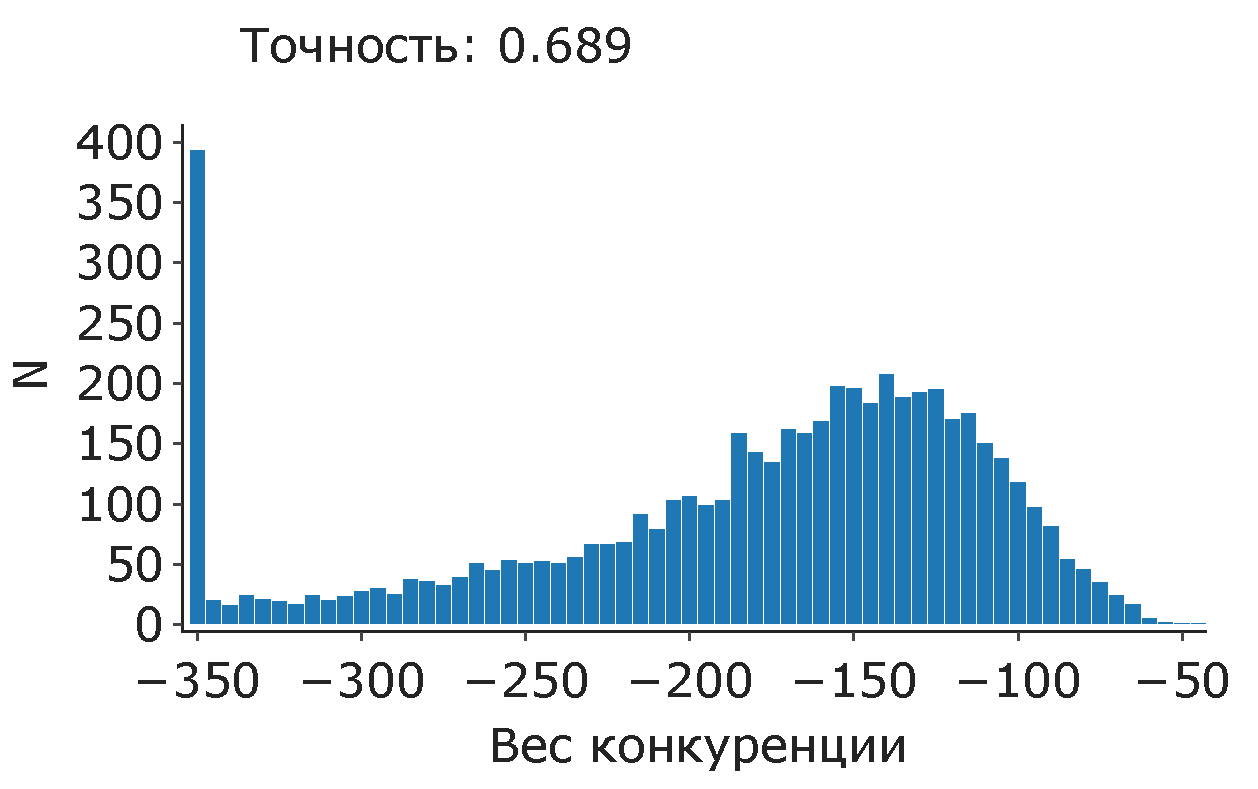
\includegraphics[width=\textwidth,keepaspectratio=true]{competition_distribution_clamp_low_ru.pdf}
    \caption{Распределение весов конкуренции, ограничение сверху} 
\end{subfigure}
\begin{subfigure}{0.45\textwidth}
    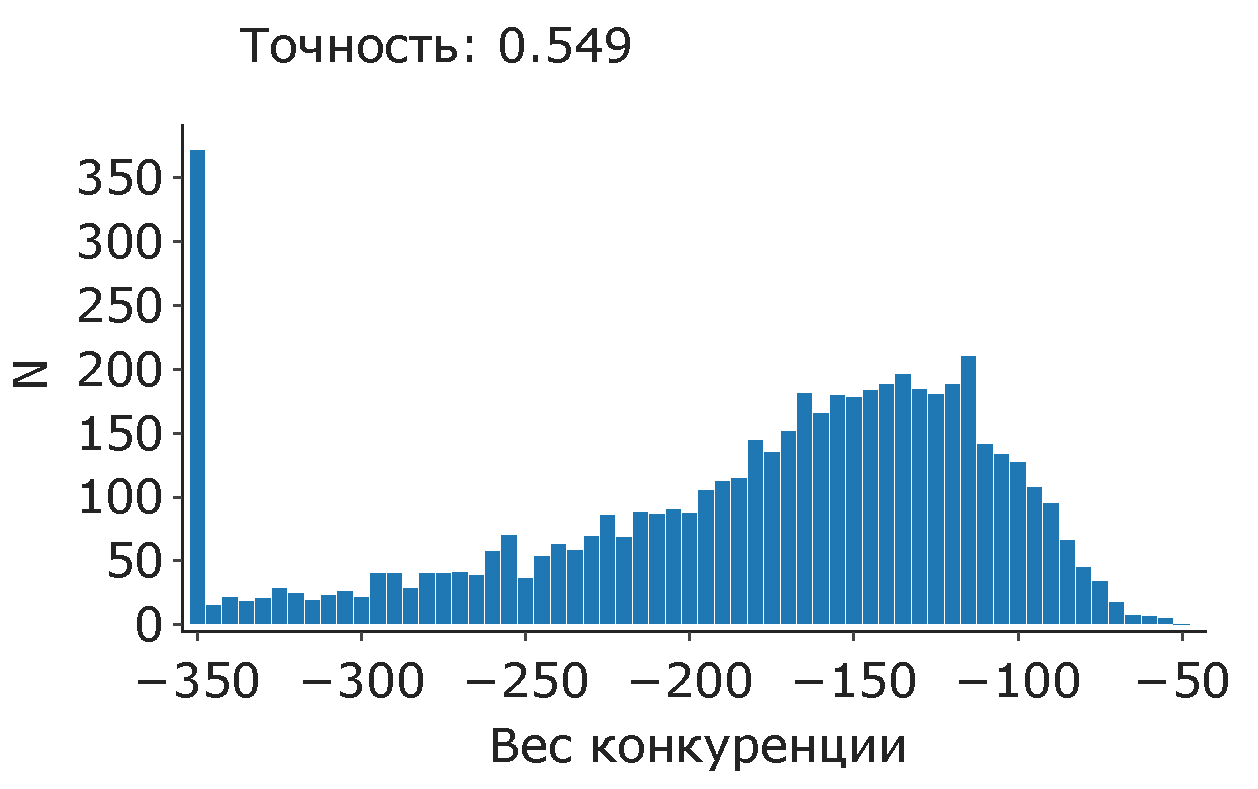
\includegraphics[width=\textwidth,keepaspectratio=true]{competition_distribution_clamp_high_ru.pdf}
    \caption{Распределение весов конкуренции, ограничение снизу}
\end{subfigure}
\begin{subfigure}{0.45\textwidth}
    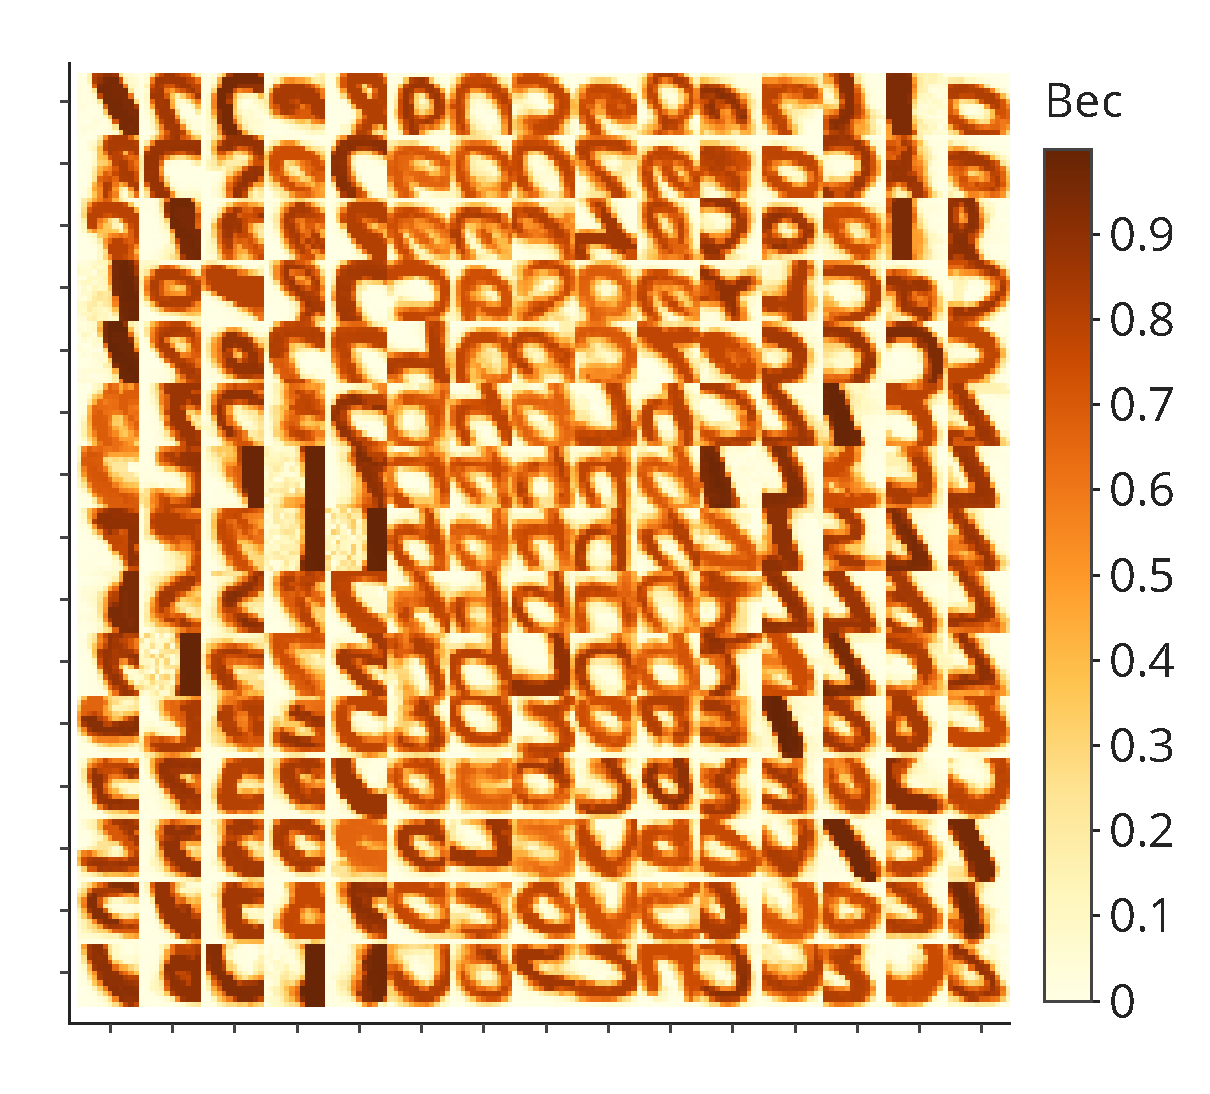
\includegraphics[width=\textwidth,keepaspectratio=true]{weights_XY_clamp_low_ru.pdf}
    \caption{Веса прямого распространения, ограничение сверху}
\end{subfigure} 
\begin{subfigure}{0.45\textwidth}
    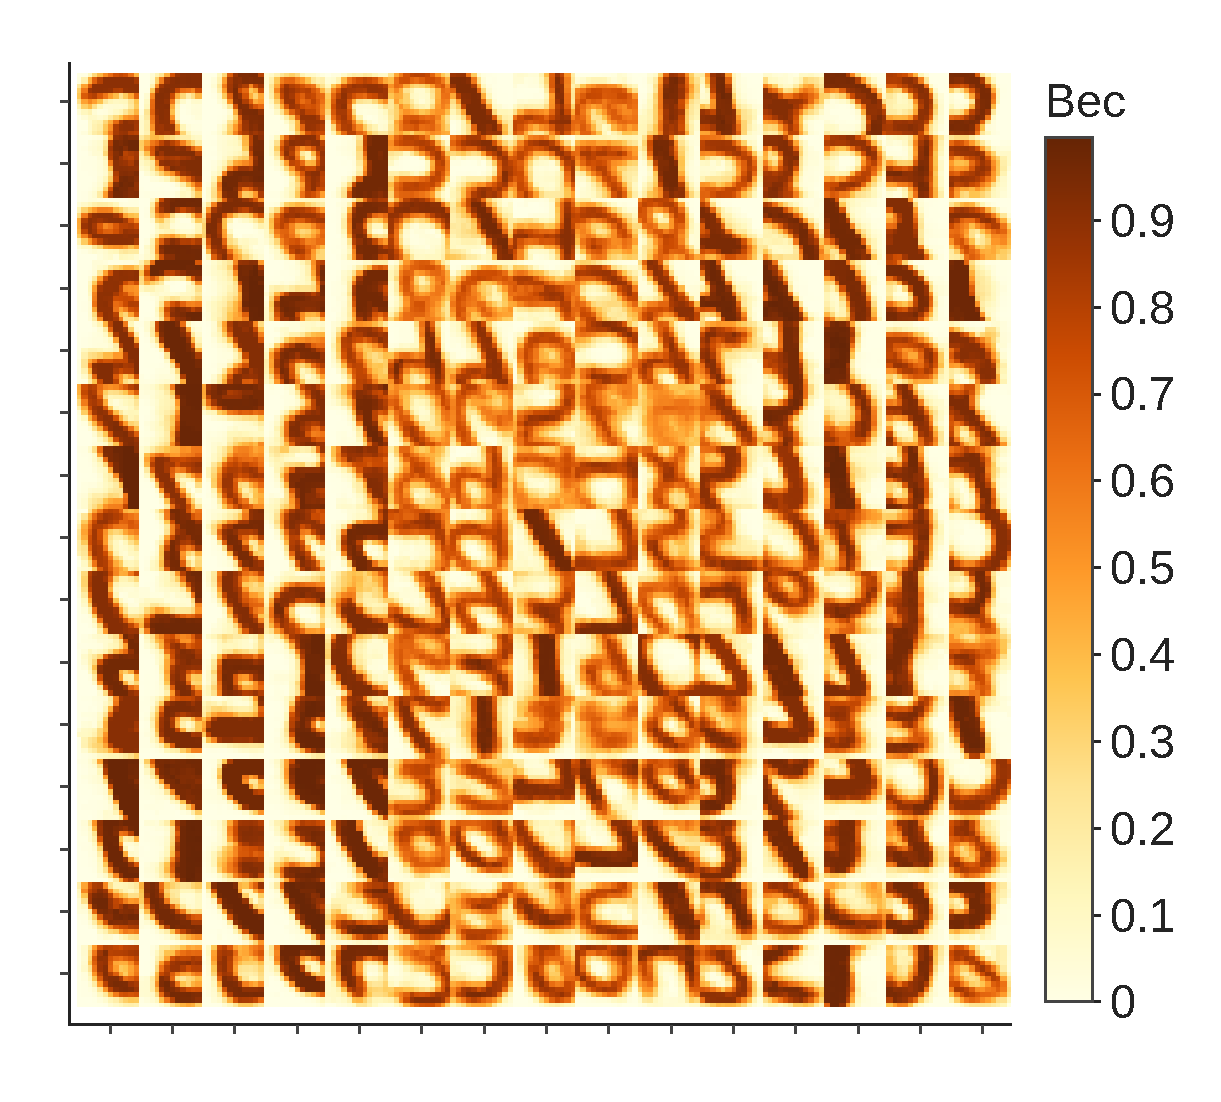
\includegraphics[width=\textwidth,keepaspectratio=true]{weights_XY_clamp_high_ru.pdf}
    \caption{Веса прямого распространения, ограничение снизу}
\end{subfigure} 
\caption{Влияние ограничения значений весов конкуренции на точность. Веса были ограничены значениями $-350$ снизу и $-100$ сверху. Точность сети с аналогичными параметрами, но без ограничения конкуренции составляет 0.823, ее веса $XY$ изображены на Рис. \ref{fig:best_competition_XY}, а распределение ее весов конкуренции --- на Рис. \ref{fig:best_competition}. Видно, что в обоих случаях обучаются менее четкие веса прямого распространения.}
\label{fig:compe_clamp}
\end{figure}

Обучение конкуренции позволило достичь точности, незначительно (на 2\%) превышающей точность сети такой же конфигурации, но с фиксированной конкуренцией с ингибирующими весами, равными $-50$ (Таб. \ref{results}, №4 и №5). 

\section{Обсуждение}
Настоящее исследование демонстрирует, что локально соединенная сеть – перспективная спайковая нейросетевая архитектура, подходящая для эффективной реализации на специализированном нейрочипе. Действительно, способность быстро выходить на плато кривой обучения позволяет использовать LCSNN для обучения на выборках сравнительно небольшого объема (3000-5000). Использование дополнительного алгоритма интерпретации активности, такого как линейный классификатор, позволяет повысить эффективность сети. Заметим, что при этом сами признаки распознаваемых объектов выучиваются сетью без учителя. Остается открытым вопрос о возможности получения схожих результатов без использования обучения с учителем для интерпретации активности сети.

Главным преимуществом LCSNN является, как было показано, то, что локально соединенная сеть превосходит сверточную в точности при примерно одинаковом или чуть большем числе параметров. Предположительно, это происходит за счет более богатой статистики патчей (рецептивных полей), на которые реагируют нейроны внутри каждого канала, по сравнению с одним рецептивным полем на каждый канал в сверточной архитектуре. Ценой за это является увеличенное число параметров в LCSNN, но не является критическим фактором, ввиду локальной (в противоположность полносвязной) топологии межнейронных контактов. Локальная архитектура также позволяет сохранить информацию о локализации выделяемого признака в пространстве и потому является разумным выбором для реализации SNN, обучающихся преимущественно без учителя. Данный выбор обусловливает также его совокупную эффективность (по производимости, точности и энергопотреблению при определённой плотности элементов) при аппаратной реализации, при которой каждый вес обычно представлен одним или несколькими физическими элементами (главным образом, ячейками SRAM \cite{TrueNorth, Loihi} или мемристорами \cite{Li_2018}).
Обучение связей конкуренции слегка увеличивает точность работы алгоритма на базе LCSNN, но не настолько критично, чтобы оправдывать использование такой дорогой операции как введение и обучение значительного числа ингибирующих связей с различными по модулю конечными весами. В то же время, вероятно, этот вывод справедлив только для небольших сетей, вроде исследованной в настоящей работе. На наш взгляд, более тщательного изучения заслуживает подбор оптимальных алгоритмов и параметров обучения конкуренции для глубоких SNN, в которых баланс конкуренции и кооперации нейронов внутри каждого слоя может приводить к формированию кластеров из классов подаваемых изображений, что способствует выстраиванию семантически-подобной иерархии выученных признаков и их комбинаций, то есть конечных образов \cite{10.1007/978-3-030-30425-6_30}. Потенциально такая иерархия образов может привести к существенному приросту качественных показателей работы интеллектуальных алгоритмов. 

\clearpage
\addcontentsline{toc}{section}{Выводы}
\section*{Выводы}
Было показано, что для задачи распознавания образов на датасете MNIST локально соединенная архитектура с конкуренцией превосходит сверточную при равном числе параметров.
Также было показано, что обучение весов конкуренции позволяет незначительно повысить качество модели, а в полученном распределении весов конкуренции важны как высокие по модулю (сильная конкуренция), так и низкие (кооперация) значения весов.


\printbibliography[sorting=none,heading=bibintoc,type=article,title={Литература}]
 
\begin{center}
Все материалы этой работы находятся в репозитории\\
\href{https://github.com/danielgafni/bachelor}{https://github.com/danielgafni/bachelor} 
\end{center}

\end{document}  
